\documentclass[output=paper,hidelinks]{langscibook}
\ChapterDOI{10.5281/zenodo.10185980}
\title{LFG, Optimality Theory and learnability of languages}
\author{Jonas Kuhn\affiliation{University of Stuttgart}}
\abstract{Optimality-Theoretic accounts of grammar specification do not rely (exclusively) on rules and descriptions that every expression in the implied formal language has to satisfy strictly. Instead, a universal set of violable constraints is posited, and most grammatical expressions are not perfectly harmonic in all respects, but violate some of the constraints. A particular language is characterized by a certain priority ranking over the universal constraint set. This conceptualization of grammatical knowledge gives rise to the prediction of cross-linguistic variation: across languages, the same underlying meaning is realized by different expressions since different rankings of the constraints make different candidates optimal. The framework comes with a straightforward algorithmic formulation of the language learning problem -- as error-driven constraint reranking.

Optimality Theory (OT) was combined with many linguistic description frameworks in the 1990s. LFG turned out to be a very appropriate base formalism for specifying the candidate representations in OT's competition-based definition of grammaticality. The novel way of characterizing formal languages prompted a range of debates regarding central assumptions in linguistic theorizing; various extensions of the competition-based setup were proposed; and the concept of violable constraints was taken over as an effective modeling device for managing ambiguities in broad-coverage computational grammar development. This chapter provides an introduction of the core concepts of OT as fleshed out on the basis of LFG, it illustrates the most influential extensions,  and it reviews important conceptual debates triggered by the approach.
}

\IfFileExists{../localcommands.tex}{
   \addbibresource{../localbibliography.bib}
   \addbibresource{thisvolume.bib}
   % add all extra packages you need to load to this file

\usepackage{tabularx}
\usepackage{multicol}
\usepackage{url}
\urlstyle{same}
%\usepackage{amsmath,amssymb}

% Tight underlining according to https://alexwlchan.net/2017/10/latex-underlines/
\usepackage{contour}
\usepackage[normalem]{ulem}
\renewcommand{\ULdepth}{1.8pt}
\contourlength{0.8pt}
\newcommand{\tightuline}[1]{%
  \uline{\phantom{#1}}%
  \llap{\contour{white}{#1}}}
  
\usepackage{listings}
\lstset{basicstyle=\ttfamily,tabsize=2,breaklines=true}

% \usepackage{langsci-basic}
\usepackage{langsci-optional}
\usepackage[danger]{langsci-lgr}
\usepackage{langsci-gb4e}
%\usepackage{langsci-linguex}
%\usepackage{langsci-forest-setup}
\usepackage[tikz]{langsci-avm} % added tikz flag, 29 July 21
% \usepackage{langsci-textipa}

\usepackage[linguistics,edges]{forest}
\usepackage{tikz-qtree}
\usetikzlibrary{positioning, tikzmark, arrows.meta, calc, matrix, shapes.symbols}
\usetikzlibrary{arrows, arrows.meta, shapes, chains, decorations.text}

%%%%%%%%%%%%%%%%%%%%% Packages for all chapters

% arrows and lines between structures
\usepackage{pst-node}

% lfg attributes and values, lines (relies on pst-node), lexical entries, phrase structure rules
\usepackage{packages/lfg-abbrevs}

% subfigures
\usepackage{subcaption}

% macros for small illustrations in the glossary
\usepackage{./packages/picins}

%%%%%%%%%%%%%%%%%%%%% Packages from contributors

% % Simpler Syntax packages
\usepackage{bm}
\tikzstyle{block} = [rectangle, draw, text width=5em, text centered, minimum height=3em]
\tikzstyle{line} = [draw, thick, -latex']

% Dependency packages
\usepackage{tikz-dependency}
%\usepackage{sdrt}

\usepackage{soul}

\usepackage[notipa]{ot-tableau}

% Historical
\usepackage{stackengine}
\usepackage{bigdelim}

% Morphology
\usepackage{./packages/prooftree}
\usepackage{arydshln}
\usepackage{stmaryrd}

% TAG
\usepackage{pbox}

\usepackage{langsci-branding}

   % %%%%%%%%% lang sci press commands

\newcommand*{\orcid}{}

\makeatletter
\let\thetitle\@title
\let\theauthor\@author
\makeatother

\newcommand{\togglepaper}[1][0]{
   \bibliography{../localbibliography}
   \papernote{\scriptsize\normalfont
     \theauthor.
     \titleTemp.
     To appear in:
     Dalrymple, Mary (ed.).
     Handbook of Lexical Functional Grammar.
     Berlin: Language Science Press. [preliminary page numbering]
   }
   \pagenumbering{roman}
   \setcounter{chapter}{#1}
   \addtocounter{chapter}{-1}
}

\DeclareOldFontCommand{\rm}{\normalfont\rmfamily}{\mathrm}
\DeclareOldFontCommand{\sf}{\normalfont\sffamily}{\mathsf}
\DeclareOldFontCommand{\tt}{\normalfont\ttfamily}{\mathtt}
\DeclareOldFontCommand{\bf}{\normalfont\bfseries}{\mathbf}
\DeclareOldFontCommand{\it}{\normalfont\itshape}{\mathit}
\makeatletter
\DeclareOldFontCommand{\sc}{\normalfont\scshape}{\@nomath\sc}
\makeatother

% Bug fix, 3 April 2021
\SetupAffiliations{output in groups = false,
                   separator between two = {\bigskip\\},
                   separator between multiple = {\bigskip\\},
                   separator between final two = {\bigskip\\}
                   }

% commands for all chapters
\setmathfont{LibertinusMath-Additions.otf}[range="22B8]

% punctuation between a sequence of years in a citation
% OLD: \renewcommand{\compcitedelim}{\multicitedelim}
\renewcommand{\compcitedelim}{\addcomma\space}

% \citegen with no parentheses around year
\providecommand{\citegenalt}[2][]{\citeauthor{#2}'s \citeyear*[#1]{#2}}

% avms with plain font, using langsci-avm package
\avmdefinestyle{plain}{attributes=\normalfont,values=\normalfont,types=\normalfont,extraskip=0.2em}
% avms with attributes and values in small caps, using langsci-avm package
\avmdefinestyle{fstr}{attributes=\scshape,values=\scshape,extraskip=0.2em}
% avms with attributes in small caps, values in plain font (from peter sells)
\avmdefinestyle{fstr-ps}{attributes=\scshape,values=\normalfont,extraskip=0.2em}

% reference to previous or following examples, from Stefan
%(\mex{1}) is like \next, referring to the next example
%(\mex{0}) is like \last, referring to the previous example, etc
\makeatletter
\newcommand{\mex}[1]{\the\numexpr\c@equation+#1\relax}
\makeatother

% do not add xspace before these
\xspaceaddexceptions{1234=|*\}\restrict\,}

% Several chapters use evnup -- this is verbatim from lingmacros.sty
\makeatletter
\def\evnup{\@ifnextchar[{\@evnup}{\@evnup[0pt]}}
\def\@evnup[#1]#2{\setbox1=\hbox{#2}%
\dimen1=\ht1 \advance\dimen1 by -.5\baselineskip%
\advance\dimen1 by -#1%
\leavevmode\lower\dimen1\box1}
\makeatother

% Centered entries in tables.  Requires array package.
\newcolumntype{P}[1]{>{\centering\arraybackslash}p{#1}}

% Reference to multiple figures, requested by Victoria Rosen
\newcommand{\figsref}[2]{Figures~\ref{#1}~and~\ref{#2}}
\newcommand{\figsrefthree}[3]{Figures~\ref{#1},~\ref{#2}~and~\ref{#3}}
\newcommand{\figsreffour}[4]{Figures~\ref{#1},~\ref{#2},~\ref{#3}~and~\ref{#4}}
\newcommand{\figsreffive}[5]{Figures~\ref{#1},~\ref{#2},~\ref{#3},~\ref{#4}~and~\ref{#5}}

% Semitic chapter:
\providecommand{\textchi}{χ}

% Prosody chapter
\makeatletter
\providecommand{\leftleadsto}{%
  \mathrel{\mathpalette\reflect@squig\relax}%
}
\newcommand{\reflect@squig}[2]{%
  \reflectbox{$\m@th#1$$\leadsto$}%
}
\makeatother
\newcommand\myrotaL[1]{\mathrel{\rotatebox[origin=c]{#1}{$\leadsto$}}}
\newcommand\Prosleftarrow{\myrotaL{-135}}
\newcommand\myrotaR[1]{\mathrel{\rotatebox[origin=c]{#1}{$\leftleadsto$}}}
\newcommand\Prosrightarrow{\myrotaR{135}}

% Core Concepts chapter
\newcommand{\anterm}[2]{#1\\#2}
\newcommand{\annode}[2]{#1\\#2}

% HPSG chapter
\newcommand{\HPSGphon}[1]{〈#1〉}
% for defining RSRL relations:
\newcommand{\HPSGsfl}{\enskip\ensuremath{\stackrel{\forall{}}{\Longleftarrow{}}}\enskip}
% AVM commands, valid only inside \avm{}
\avmdefinecommand {phon}[phon] { attributes=\itshape } % define a new \phon command
% Forest Set-up
\forestset
  {notin label above/.style={edge label={node[midway,sloped,above,inner sep=0pt]{\strut$\ni$}}},
    notin label below/.style={edge label={node[midway,sloped,below,inner sep=0pt]{\strut$\ni$}}},
  }

% Dependency chapter
\newcommand{\ua}{\ensuremath{\uparrow}}
\newcommand{\da}{\ensuremath{\downarrow}}
\forestset{
  dg edges/.style={for tree={parent anchor=south, child anchor=north,align=center,base=bottom},
                 where n children=0{tier=word,edge=dotted,calign with current edge}{}
                },
dg transfer/.style={edge path={\noexpand\path[\forestoption{edge}, rounded corners=3pt]
    % the line downwards
    (!u.parent anchor)-- +($(0,-l)-(0,4pt)$)-- +($(12pt,-l)-(0,4pt)$)
    % the horizontal line
    ($(!p.north west)+(0,l)-(0,20pt)$)--($(.north east)+(0,l)-(0,20pt)$)\forestoption{edge label};},!p.edge'={}},
% for Tesniere-style junctions
dg junction/.style={no edge, tikz+={\draw (!p.east)--(!.west) (.east)--(!n.west);}    }
}


% Glossary
\makeatletter % does not work with \newcommand
\def\namedlabel#1#2{\begingroup
   \def\@currentlabel{#2}%
   \phantomsection\label{#1}\endgroup
}
\makeatother


\renewcommand{\textopeno}{ɔ}
\providecommand{\textepsilon}{ɛ}

\renewcommand{\textbari}{ɨ}
\renewcommand{\textbaru}{ʉ}
\newcommand{\acutetextbari}{í̵}
\renewcommand{\textlyoghlig}{ɮ}
\renewcommand{\textdyoghlig}{ʤ}
\renewcommand{\textschwa}{ə}
\renewcommand{\textprimstress}{ˈ}
\newcommand{\texteng}{ŋ}
\renewcommand{\textbeltl}{ɬ}
\newcommand{\textramshorns}{ɤ}

\newbool{bookcompile}
\booltrue{bookcompile}
\newcommand{\bookorchapter}[2]{\ifbool{bookcompile}{#1}{#2}}




\renewcommand{\textsci}{ɪ}
\renewcommand{\textturnscripta}{ɒ}

\renewcommand{\textscripta}{ɑ}
\renewcommand{\textteshlig}{ʧ}
\providecommand{\textupsilon}{υ}
\renewcommand{\textyogh}{ʒ}
\newcommand{\textpolhook}{̨}

\renewcommand{\sectref}[1]{Section~\ref{#1}}

%\KOMAoptions{chapterprefix=true}

\renewcommand{\textturnv}{ʌ}
\renewcommand{\textrevepsilon}{ɜ}
\renewcommand{\textsecstress}{ˌ}
\renewcommand{\textscriptv}{ʋ}
\renewcommand{\textglotstop}{ʔ}
\renewcommand{\textrevglotstop}{ʕ}
%\newcommand{\textcrh}{ħ}
\renewcommand{\textesh}{ʃ}

% label for submitted and published chapters
\newcommand{\submitted}{{\color{red}Final version submitted to Language Science Press.}}
\newcommand{\published}{{\color{red}Final version published by
    Language Science Press, available at \url{https://langsci-press.org/catalog/book/312}.}}

% Treebank definitions
\definecolor{tomato}{rgb}{0.9,0,0}
\definecolor{kelly}{rgb}{0,0.65,0}

% Minimalism chapter
\newcommand\tr[1]{$<$\textcolor{gray}{#1}$>$}
\newcommand\gapline{\lower.1ex\hbox to 1.2em{\bf \ \hrulefill\ }}
\newcommand\cnom{{\llap{[}}Case:Nom{\rlap{]}}}
\newcommand\cacc{{\llap{[}}Case:Acc{\rlap{]}}}
\newcommand\tpres{{\llap{[}}Tns:Pres{\rlap{]}}}
\newcommand\fstackwe{{\llap{[}}Tns:Pres{\rlap{]}}\\{\llap{[}}Pers:1{\rlap{]}}\\{\llap{[}}Num:Pl{\rlap{]}}}
\newcommand\fstackone{{\llap{[}}Tns:Past{\rlap{]}}\\{\llap{[}}Pers:\ {\rlap{]}}\\{\llap{[}}Num:\ {\rlap{]}}}
\newcommand\fstacktwo{{\llap{[}}Pers:3{\rlap{]}}\\{\llap{[}}Num:Pl{\rlap{]}}\\{\llap{[}}Case:\ {\rlap{]}}}
\newcommand\fstackthr{{\llap{[}}Tns:Past{\rlap{]}}\\{\llap{[}}Pers:3{\rlap{]}}\\{\llap{[}}Num:Pl{\rlap{]}}} 
\newcommand\fstackfou{{\llap{[}}Pers:3{\rlap{]}}\\{\llap{[}}Num:Pl{\rlap{]}}\\{\llap{[}}Case:Nom{\rlap{]}}}
\newcommand\fstackonefill{{\llap{[}}Tns:Past{\rlap{]}}\\{\llap{[}}Pers:3{\rlap{]}}\\%
  {\llap{[}}Num:Pl{\rlap{]}}}
\newcommand\fstackoneint%
    {{\llap{[}}{\bf Tns:Past}{\rlap{]}}\\{\llap{[}}Pers:\ {\rlap{]}}\\{\llap{[}}Num:\ {\rlap{]}}}
\newcommand\fstacktwoint%
    {{\llap{[}}{\bf Pers:3}{\rlap{]}}\\{\llap{[}}{\bf Num:Pl}{\rlap{]}}\\{\llap{[}}Case:\ {\rlap{]}}}
\newcommand\fstackthrchk%
    {{\llap{[}}{\bf Tns:Past}{\rlap{]}}\\{\llap{[}}{Pers:3}{\rlap{]}}\\%
      {\llap{[}}Num:Pl{\rlap{]}}} 
\newcommand\fstackfouchk%
    {{\llap{[}}{\bf Pers:3}{\rlap{]}}\\{\llap{[}}{\bf Num:Pl}{\rlap{]}}\\%
      {\llap{[}}Case:Nom{\rlap{]}}}
\newcommand\uinfl{{\llap{[}}Infl:\ \ {\rlap{]}}}
\newcommand\inflpass{{\llap{[}}Infl:Pass{\rlap{]}}}
\newcommand\fepp{{\llap{[}}EPP{\rlap{]}}}
\newcommand\sepp{{\llap{[}}\st{EPP}{\rlap{]}}}
\newcommand\rdash{\rlap{\hbox to 24em{\hfill (dashed lines represent
      information flow)}}}


% Computational chapter
\usepackage{./packages/kaplan}
\renewcommand{\red}{\color{lsLightWine}}

% Sinitic
\newcommand{\FRAME}{\textsc{frame}\xspace}
\newcommand{\arglistit}[1]{{\textlangle}\textit{#1}{\textrangle}}

%WestGermanic
\newcommand{\streep}[1]{\mbox{\rule{1pt}{0pt}\rule[.5ex]{#1}{.5pt}\rule{-1pt}{0pt}\rule{-#1}{0pt}}}

\newcommand{\hspaceThis}[1]{\hphantom{#1}}


\newcommand{\FIG}{\textsc{figure}}
\newcommand{\GR}{\textsc{ground}}

%%%%% Morphology
% Single quote
\newcommand{\asquote}[1]{`{#1}'} % Single quotes
\newcommand{\atrns}[1]{\asquote{#1}} % Translation
\newcommand{\attrns}[1]{(\asquote{#1})} % Translation
\newcommand{\ascare}[1]{\asquote{#1}} % Scare quotes
\newcommand{\aqterm}[1]{\asquote{#1}} % Quoted terms
% Double quote
\newcommand{\adquote}[1]{``{#1}''} % Double quotes
\newcommand{\aquoot}[1]{\adquote{#1}} % Quotes
% Italics
\newcommand{\aword}[1]{\textit{#1}}  % mention of word
\newcommand{\aterm}[1]{\textit{#1}}
% Small caps
\newcommand{\amg}[1]{{\textsc{\MakeLowercase{#1}}}}
\newcommand{\ali}[1]{\MakeLowercase{\textsc{#1}}}
\newcommand{\feat}[1]{{\textsc{#1}}}
\newcommand{\val}[1]{\textsc{#1}}
\newcommand{\pred}[1]{\textsc{#1}}
\newcommand{\predvall}[1]{\textsc{#1}}
% Misc commands
\newcommand{\exrr}[2][]{(\ref{ex:#2}{#1})}
\newcommand{\csn}[3][t]{\begin{tabular}[#1]{@{\strut}c@{\strut}}#2\\#3\end{tabular}}
\newcommand{\sem}[2][]{\ensuremath{\left\llbracket \mbox{#2} \right\rrbracket^{#1}}}
\newcommand{\apf}[2][\ensuremath{\sigma}]{\ensuremath{\langle}#2,#1\ensuremath{\rangle}}
\newcommand{\formula}[2][t]{\ensuremath{\begin{array}[#1]{@{\strut}l@{\strut}}#2%
                                         \end{array}}}
\newcommand{\Down}{$\downarrow$}
\newcommand{\Up}{$\uparrow$}
\newcommand{\updown}{$\uparrow=\downarrow$}
\newcommand{\upsigb}{\mbox{\ensuremath{\uparrow\hspace{-0.35em}_\sigma}}}
\newcommand{\lrfg}{L\textsubscript{R}FG} 
\newcommand{\dmroot}{\ensuremath{\sqrt{\hspace{1em}}}}
\newcommand{\amother}{\mbox{\ensuremath{\hat{\raisebox{-.25ex}{\ensuremath{\ast}}}}}}
\newcommand{\expone}{\ensuremath{\xrightarrow{\nu}}}
\newcommand{\sig}{\mbox{$_\sigma\,$}}
\newcommand{\aset}[1]{\{#1\}}
\newcommand{\linimp}{\mbox{\ensuremath{\,\multimap\,}}}
\newcommand{\fsfunc}{\ensuremath{\Phi}\hspace*{-.15em}}
\newcommand{\cons}[1]{\ensuremath{\mbox{\textbf{\textup{#1}}}}}
\newcommand{\amic}[1][]{\cons{MostInformative$_c$}{#1}}
\newcommand{\amif}[1][]{\cons{MostInformative$_f$}{#1}}
\newcommand{\amis}[1][]{\cons{MostInformative$_s$}{#1}}
\newcommand{\amsp}[1][]{\cons{MostSpecific}{#1}}

%Glue
\newcommand{\glues}{Glue Semantics} % macro for consistency
\newcommand{\glue}{Glue} % macro for consistency
\newcommand{\lfgglue}{LFG$+$Glue} 
\newcommand{\scare}[1]{`{#1}'} % Scare quotes
\newcommand{\word}[1]{\textit{#1}}  % mention of word
\newcommand{\dquote}[1]{``{#1}''} % Double quotes
\newcommand{\high}[1]{\textit{#1}} % highlight (italicize)
\newcommand{\laml}{{L}} 
% Left interpretation double bracket
\newcommand{\Lsem}{\ensuremath{\left\llbracket}} 
% Right interpretation double bracket
\newcommand{\Rsem}{\ensuremath{\right\rrbracket}} 
\newcommand{\nohigh}[1]{{#1}} % nohighlight (regular font)
% Linear implication elimination
\newcommand{\linimpE}{\mbox{\small\ensuremath{\multimap_{\mathcal{E}}}}}
% Linear implication introduction, plain
\newcommand{\linimpI}{\mbox{\small\ensuremath{\multimap_{\mathcal{I}}}}}
% Linear implication introduction, with flag
\newcommand{\linimpIi}[1]{\mbox{\small\ensuremath{\multimap_{{\mathcal{I}},#1}}}}
% Linear universal elimination
\newcommand{\forallE}{\mbox{\small\ensuremath{\forall_{{\mathcal{E}}}}}}
% Tensor elimination
\newcommand{\tensorEij}[2]{\mbox{\small\ensuremath{\otimes_{{\mathcal{E}},#1,#2}}}}
% CG forward slash
\newcommand{\fs}{\ensuremath{/}} 
% s-structure mapping, no space after                                     
\newcommand{\sigb}{\mbox{$_\sigma$}}
% uparrow with s-structure mapping, with small space after  
\newcommand{\upsig}{\mbox{\ensuremath{\uparrow\hspace{-0.35em}_\sigma\,}}}
\newcommand{\fsa}[1]{\textit{#1}}
\newcommand{\sqz}[1]{#1}
% Angled brackets (types, etc.)
\newcommand{\bracket}[1]{\ensuremath{\left\langle\mbox{\textit{#1}}\right\rangle}}
% glue logic string term
\newcommand{\gterm}[1]{\ensuremath{\mbox{\textup{\textit{#1}}}}}
% abstract grammatical formative
\newcommand{\gform}[1]{\ensuremath{\mbox{\textsc{\textup{#1}}}}}
% let
\newcommand{\llet}[3]{\ensuremath{\mbox{\textsf{let}}~{#1}~\mbox{\textsf{be}}~{#2}~\mbox{\textsf{in}}~{#3}}}
% Word-adorned proof steps
\providecommand{\vformula}[2]{%
  \begin{array}[b]{l}
    \mbox{\textbf{\textit{#1}}}\\%[-0.5ex]
    \formula{#2}
  \end{array}
}

%TAG
\newcommand{\fm}[1]{\textsc{#1}}
\newcommand{\struc}[1]{{#1-struc\-ture}}
\newcommand{\func}[1]{\mbox{#1-function}}
\newcommand{\fstruc}{\struc{f}}
\newcommand{\cstruc}{\struc{c}}
\newcommand{\sstruc}{\struc{s}}
\newcommand{\astruc}{\struc{a}}
\newcommand{\nodelabels}[2]{\rlap{\ensuremath{^{#1}_{#2}}}}
\newcommand{\footnode}{\rlap{\ensuremath{^{*}}}}
\newcommand{\nafootnode}{\rlap{\ensuremath{^{*}_{\nalabel}}}}
\newcommand{\nanode}{\rlap{\ensuremath{_{\nalabel}}}}
\newcommand{\AdjConstrText}[1]{\textnormal{\small #1}}
\newcommand{\nalabel}{\AdjConstrText{NA}}

%Case
\newcommand{\MID}{\textsc{mid}{}\xspace}

%font commands added April 2023 for Control and Case chapters
\def\textthorn{þ}
\def\texteth{ð}
\def\textinvscr{ʁ}
\def\textcrh{ħ}
\def\textgamma{ɣ}

% Coordination
\newcommand{\CONJ}{\textsc{conj}{}\xspace}
\newcommand*{\phtm}[1]{\setbox0=\hbox{#1}\hspace{\wd0}}
\newcommand{\ggl}{\hfill(Google)}
\newcommand{\nkjp}{\hfill(NKJP)}

% LDDs
\newcommand{\ubd}{\attr{ubd}\xspace}
% \newcommand{\disattr}[1]{\blue \attr{#1}}  % on topic/focus path
% \newcommand{\proattr}[1]{\green\attr{#1}}  % On Q/Relpro path
\newcommand{\disattr}[1]{\color{lsMidBlue}\attr{#1}}  % on topic/focus path
\newcommand{\proattr}[1]{\color{lsMidGreen}\attr{#1}}  % On Q/Relpro path
\newcommand{\eestring}{\mbox{$e$}\xspace}
\providecommand{\disj}[1]{\{\attr{#1}\}}
\providecommand{\estring}{\mb{\epsilon}}
\providecommand{\termcomp}[1]{\attr{\backslash {#1}}}
\newcommand{\templatecall}[2]{{\small @}(\attr{#1}\ \attr{#2})}
\newcommand{\xlgf}[1]{(\leftarrow\ \attr{#1})} 
\newcommand{\xrgf}[1]{(\rightarrow\ \attr{#1})}
\newcommand{\rval}[2]{\annobox {\xrgf{#1}\teq\attr{#2}}}
\newcommand{\memb}[1]{\annobox {\downarrow\, \in \xugf{#1}}}
\newcommand{\lgf}[1]{\annobox {\xlgf{#1}}}
\newcommand{\rgf}[1]{\annobox {\xrgf{#1}}}
\newcommand{\rvalc}[2]{\annobox {\xrgf{#1}\teqc\attr{#2}}}
\newcommand{\xgfu}[1]{(\attr{#1}\uparrow)}
\newcommand{\gfu}[1]{\annobox {\xgfu{#1}}}
\newcommand{\nmemb}[3]{\annobox {{#1}\, \in \ngf{#2}{#3}}}
\newcommand{\dgf}[1]{\annobox {\xdgf{#1}}}
\newcommand{\predsfraise}[3]{\annobox {\xugf{pred}\teq\semformraise{#1}{#2}{#3}}}
\newcommand{\semformraise}[3]{\annobox {\textrm{`}\hspace{-.05em}\attr{#1}\langle\attr{#2}\rangle{\attr{#3}}\textrm{'}}}
\newcommand{\teqc}{\hspace{-.1667em}=_c\hspace{-.1667em}} 
\newcommand{\lval}[2]{\annobox {\xlgf{#1}\teq\attr{#2}}}
\newcommand{\xgfd}[1]{(\attr{#1}\downarrow)}
\newcommand{\gfd}[1]{\annobox {\xgfd{#1}}}
\newcommand{\gap}{\rule{.75em}{.5pt}\ }
\newcommand{\gapp}{\rule{.75em}{.5pt}$_p$\ }

% Mapping
% Avoid having to write 'argument structure' a million times
\newcommand{\argstruc}{argument structure}
\newcommand{\Argstruc}{Argument structure}
\newcommand{\emptybracks}{\ensuremath{[\;\;]}}
\newcommand{\emptycurlybracks}{\ensuremath{\{\;\;\}}}
% Drawing lines in structures
\newcommand{\strucconnect}[6]{%
\draw[-stealth] (#1) to[out=#5, in=#6] node[pos=#3, above]{#4} (#2);%
}
\newcommand{\strucconnectdashed}[6]{%
\draw[-stealth, dashed] (#1) to[out=#5, in=#6] node[pos=#3, above]{#4} (#2);%
}
% Attributes for s-structures in the style of lfg-abbrevs.sty
\newcommand{\ARGnum}[1]{\textsc{arg}\textsubscript{#1}}
% Drawing mapping lines
\newcommand{\maplink}[2]{%
\begin{tikzpicture}[baseline=(A.base)]
\node(A){#1\strut};
\node[below = 3ex of A](B){\pbox{\textwidth}{#2}};
\draw ([yshift=-1ex]A.base)--(B);
% \draw (A)--(B);
\end{tikzpicture}}
% long line for extra features
\newcommand{\longmaplink}[2]{%
\begin{tikzpicture}[baseline=(A.base)]
\node(A){#1\strut};
\node[below = 3ex of A](B){\pbox{\textwidth}{#2}};
\draw ([yshift=2.5ex]A.base)--(B);
% \draw (A)--(B);
\end{tikzpicture}%
}
% For drawing upward
\newcommand{\maplinkup}[2]{%
\begin{tikzpicture}[baseline=(A.base)]
\node(A){#1};
\node[above = 3ex of A, anchor=base](B){#2};
\draw (A)--(B);
\end{tikzpicture}}
% Above with arrow going down (for argument adding processes)
\newcommand{\argumentadd}[2]{%
\begin{tikzpicture}[baseline=(A.base)]
\node(A){#1};
\node[above = 3ex of A, anchor=base](B){#2};
\draw[latex-] ([yshift=2ex]A.base)--([yshift=-1ex]B.center);
\end{tikzpicture}}
% Going up to the left
\newcommand{\maplinkupleft}[2]{%
\begin{tikzpicture}[baseline=(A.base)]
\node(A){#1};
\node[above left = 3ex of A, anchor=base](B){#2};
\draw (A)--(B);
\end{tikzpicture}}
% Going up to the right
\newcommand{\maplinkupright}[2]{%
\begin{tikzpicture}[baseline=(A.base)]
\node(A){#1};
\node[above right = 3ex of A, anchor=base](B){#2};
\draw (A)--(B);
\end{tikzpicture}}
% Argument fusion
\newenvironment{tikzsentence}{\begin{tikzpicture}[baseline=0pt, 
  anchor=base, outer sep=0pt, ampersand replacement=\&
   ]}{\end{tikzpicture}}
\newcommand{\Subnode}[2]{\subnode[inner sep=1pt]{#1}{#2\strut}}
\newcommand{\connectbelow}[3]{\draw[inner sep=0pt] ([yshift=0.5ex]#1.south) -- ++ (south:#3ex)
  -| ([yshift=0.5ex]#2.south);}
\newcommand{\connectabove}[3]{\draw[inner sep=0pt] ([yshift=0ex]#1.north) -- ++ (north:#3ex)
  -| ([yshift=0ex]#2.north);}
  
\newcommand{\ASNode}[2]{\tikz[remember picture,baseline=(#1.base)] \node [anchor=base] (#1) {#2};}

% Austronesian
\newcommand{\LV}{\textsc{lv}\xspace}
\newcommand{\IV}{\textsc{iv}\xspace}
\newcommand{\DV}{\textsc{dv}\xspace}
\newcommand{\PV}{\textsc{pv}\xspace}
\newcommand{\AV}{\textsc{av}\xspace}
\newcommand{\UV}{\textsc{uv}\xspace}

\apptocmd{\appendix}
         {\bookmarksetup{startatroot}}
         {}
         {%
           \AtEndDocument{\typeout{langscibook Warning:}
                          \typeout{It was not possible to set option 'staratroot'}
                          \typeout{for appendix in the backmatter.}}
         }

   %% hyphenation points for line breaks
%% Normally, automatic hyphenation in LaTeX is very good
%% If a word is mis-hyphenated, add it to this file
%%
%% add information to TeX file before \begin{document} with:
%% %% hyphenation points for line breaks
%% Normally, automatic hyphenation in LaTeX is very good
%% If a word is mis-hyphenated, add it to this file
%%
%% add information to TeX file before \begin{document} with:
%% %% hyphenation points for line breaks
%% Normally, automatic hyphenation in LaTeX is very good
%% If a word is mis-hyphenated, add it to this file
%%
%% add information to TeX file before \begin{document} with:
%% \include{localhyphenation}
\hyphenation{
Aus-tin
Bel-ya-ev
Bres-nan
Chom-sky
Eng-lish
Geo-Gram
INESS
Inkelas
Kaplan
Kok-ko-ni-dis
Lacz-kó
Lam-ping
Lu-ra-ghi
Lund-quist
Mcho-mbo
Meu-rer
Nord-lin-ger
PASSIVE
Pa-no-va
Pol-lard
Pro-sod-ic
Prze-piór-kow-ski
Ram-chand
Sa-mo-ye-dic
Tsu-no-da
WCCFL
Wam-ba-ya
Warl-pi-ri
Wes-coat
Wo-lof
Zae-nen
accord-ing
an-a-phor-ic
ana-phor
christ-church
co-description
co-present
con-figur-ation-al
in-effa-bil-ity
mor-phe-mic
mor-pheme
non-com-po-si-tion-al
pros-o-dy
referanse-grammatikk
rep-re-sent
Schätz-le
term-hood
Kip-ar-sky
Kok-ko-ni
Chi-che-\^wa
au-ton-o-mous
Al-si-na
Ma-tsu-mo-to
}

\hyphenation{
Aus-tin
Bel-ya-ev
Bres-nan
Chom-sky
Eng-lish
Geo-Gram
INESS
Inkelas
Kaplan
Kok-ko-ni-dis
Lacz-kó
Lam-ping
Lu-ra-ghi
Lund-quist
Mcho-mbo
Meu-rer
Nord-lin-ger
PASSIVE
Pa-no-va
Pol-lard
Pro-sod-ic
Prze-piór-kow-ski
Ram-chand
Sa-mo-ye-dic
Tsu-no-da
WCCFL
Wam-ba-ya
Warl-pi-ri
Wes-coat
Wo-lof
Zae-nen
accord-ing
an-a-phor-ic
ana-phor
christ-church
co-description
co-present
con-figur-ation-al
in-effa-bil-ity
mor-phe-mic
mor-pheme
non-com-po-si-tion-al
pros-o-dy
referanse-grammatikk
rep-re-sent
Schätz-le
term-hood
Kip-ar-sky
Kok-ko-ni
Chi-che-\^wa
au-ton-o-mous
Al-si-na
Ma-tsu-mo-to
}

\hyphenation{
Aus-tin
Bel-ya-ev
Bres-nan
Chom-sky
Eng-lish
Geo-Gram
INESS
Inkelas
Kaplan
Kok-ko-ni-dis
Lacz-kó
Lam-ping
Lu-ra-ghi
Lund-quist
Mcho-mbo
Meu-rer
Nord-lin-ger
PASSIVE
Pa-no-va
Pol-lard
Pro-sod-ic
Prze-piór-kow-ski
Ram-chand
Sa-mo-ye-dic
Tsu-no-da
WCCFL
Wam-ba-ya
Warl-pi-ri
Wes-coat
Wo-lof
Zae-nen
accord-ing
an-a-phor-ic
ana-phor
christ-church
co-description
co-present
con-figur-ation-al
in-effa-bil-ity
mor-phe-mic
mor-pheme
non-com-po-si-tion-al
pros-o-dy
referanse-grammatikk
rep-re-sent
Schätz-le
term-hood
Kip-ar-sky
Kok-ko-ni
Chi-che-\^wa
au-ton-o-mous
Al-si-na
Ma-tsu-mo-to
}

   \togglepaper[24]%%chapternumber
}{}

\begin{document}
\maketitle
\label{chap:OT}

\section{Introduction} 
\label{sec:OT:intro}

The term Optimality Theory (OT) refers to a family of grammatical frameworks developed in various subfields of linguistics following the original proposal for phonology by \citet{PrinceSmolensky1993}. %\todo{double check which version of PS93 to cite}
\citet{Bresnan-96-LFG-conference}, in her keynote address at the first LFG conference,\footnote{Details of the analysis presented in the keynote address are discussed in \citet{Bresnan-Explaining-Morphosyntactic} and \citet{Bresnan-Lexicon-in-OT}.} showed that LFG constitutes a natural base formalism for an OT account of syntax, laying the foundation for substantial research activities in the late 1990s and early 2000s.

The key idea behind OT is that grammatical knowledge is not captured in distinct rule systems for each language, but theorists assume a universal set of constraints responsible for determining the harmony or markedness of potential realizations of some underlying input representation. For example, both the clause structure \emph{you see who?} and \emph{who do you see?} are candidate realizations for expressing a \emph{wh}-question that asks for the object of a transitive verb. In some languages, the equivalent of the former is grammatical, whereas in English, the latter is. Neither of the two variants is perfectly unmarked; each violates certain constraints (in essence: an interrogative phrase is best realized at the beginning of the clause vs.\ the object of a verb is best realized in the canonical VP-internal complement position).
What differs across languages is the relative prominence among the universal constraints, such that there are different winners in the competition for the most harmonic/least marked candidate, which is defined to be the language-particular output. Learning a language thus amounts to determining the correct prominence ranking over a known set of constraints to replicate the behavior observed in adult speakers. A more technical illustration of an OT system building on the LFG formalism will follow in \sectref{sec:OT:initial-example}.

The notion of violable grammar constraints inspired linguists to explore the explanatory potential of a competition-based definition of grammaticality for a whole range of linguistic subfields. 
Moreover as  \sectref{sec:OT:OT-style-initial-example} will discuss, the notion turned out fruitful for computational work aiming at linguistically grounded broad-coverage grammars:
expanding ``classical'' constraint-based grammar formalisms with a novel type of violable constraints enables a competition-based filtering of ambiguity sources and thus greatly facilitates the treatment of relatively rare lexical variants and grammatical constructions \citep{franketal01}.
An outline of the remaining sections of this chapter will be provided in \sectref{sec:OT:chapter-outline}. %% \todo{state mission for this ch.?}

\subsection{Example of an OT-LFG analysis}
\label{sec:OT:initial-example}

The tableau in \figref{fig:tableau1} demonstrates more technically how an OT-LFG account predicts \emph{who will she see?} to be the grammatical structure for realizing this type of question in English. It is adapted from \citet{Bresnan-Explaining-Morphosyntactic}, a contribution that recasts Grimshaw's (\citeyear{Grimshaw97})  OT analysis of English verb inversion in an LFG framework assuming Extended Head Theory (as detailed in \citealt[ch.~7]{bresnan2001lexical} and \citealt[ch.~7]{BresnanEtAl2016}). 


\begin{figure}
\ShadingOn
\begin{tableau}{c|c|c}
\inp{Input: $\left[\begin{array}{ll}
\textsc{pred} & \textrm{`see(x, y)'} \\
\textsc{gf}_1 & [ \textrm{``you''}] \\
\textsc{gf}_2 & \rnode{A}{[ \textrm{``who''}]} \\
\textsc{q-foc} &  \rnode{B}{} \\
\textsc{tns} & \textsc{fut} \\
  \end{array}\right]$
  \CURVE[1]{-2pt}{0}{A}{-2pt}{0}{B}
}   \const{Op-Spec} \const{Ob-Hd} \const{Stay} 
\cand*{$\langle$ [$_\textrm{IP}$ you will [$_\textrm{VP}$ see who ]], \dots $\rangle$} \vio{*!} \vio{} \vio{}
\cand*{$\langle$ [$_\textrm{CP}$ who \emph{e} [$_\textrm{IP}$ you will [$_\textrm{VP}$ see \emph{e} ]]], \dots $\rangle$}  \vio{} \vio{*!} \vio{*}
\cand*[\HandRight]{$\langle$ [$_\textrm{CP}$ who will [$_\textrm{IP}$ you \emph{e} [$_\textrm{VP}$ see \emph{e} ]]], \dots $\rangle$} \vio{} \vio{} \vio{**}
\end{tableau}
\caption{Tableau for the competition that leads to \emph{who will you see?} being the most harmonic candidate under the constraint ranking for English. The candidates' c-structure trees are shown as bracketing expressions; their full f-structures is not shown here. Only a small subset of the candidate set is listed, omitting other realization variants. These are excluded for English by additional constraints, but could be grammatical in other languages and are thus included in the candidate set.}
\label{fig:tableau1}
\end{figure}

The tableau shows the comparison of three candidate realizations for the underlying content, the input -- here the proposition \emph{see}($x, y$), where $x$ is a pronominal for the second person singular, $y$ is the focus of a question, and the clausal realization expresses future tense. Particular syntactic choices, for instance the realization of the semantic arguments by grammatical relations such as \textsc{subject} and \textsc{object} are underspecified in the input. In the OT-LFG framework, the range of realization options across languages can be captured very well by assuming that the input is a partially specified f-structure, and the candidate set consists of all fully specified LFG analyses whose f-structure is subsumed by the input.

The excerpt from the full candidate set shown in \figref{fig:tableau1} focuses on c-struc\-tural realization alternatives for clause structure. In Extended Head Theory, functional categories (such as I and C) and their c-structure projections are mapped to the same f-structure as their corresponding lexical categories (V). The functional projections occur optionally, but they offer the possibility to realize additional head elements such as tense auxiliaries and they come with one c-structural specifier position each, which can for instance be used for \emph{wh} operators.
Also, it is a possibility across languages for verbal head elements to be realized in a higher, c-commanding, position (e.g., V in I or I in C, as in candidate c.). By definition, elements in such a functional position are still \emph{extended heads} of the lower projections. 
This nonderivational account of head mobility, which \citet[ch.~7]{bresnan2001lexical} also formalizes in a non-OT setting of LFG,  thus opens up a considerable spectrum of alternative candidate realizations for the basic clause structure. 

Let us now consider what effect the three violable constraints have that \figref{fig:tableau1} shows in the order of the ranking for English
(the constraint formalization will be discussed in more detail in \sectref{sec:OT:OT-Syntax}). The harmony/markedness of a candidate is determined by its constraint violation profile.
In the tableau notation, a violation is signalled by a star in the row for the corresponding constraint. Since OT assumes a \emph{ranking} of the constraints (and not a more general weighing as for instance in Harmonic Grammar, \citealt{Legendre-etal-1990}), one can simply proceed from left to right through the constraints to determine the winning candidate(s): at each constraint, only the candidates that have the fewest violations for this constraint are kept. The other candidates have no more chance of winning the competition, even when they do not violate any of the lower-ranking constraints.  It is common to mark the decisive constraint violations with an exclamation mark following the star; the cells for the lower-ranking constraints are often grayed out in tableaux. 
In our example competition, the \textsc{Op-Spec} constraint demands that syntactic operators such as \emph{wh} phrases be realized in c-structural specifier positions (highlighting the operator's prominence). Candidate a.\ violates this constraint, since the \emph{who} is realized inside the VP. \textsc{Op-Spec} is the highest-ranking constraint and the other candidates satisfy this constraint, hence candidate a.\ is excluded from further comparison. The \textsc{Ob-Hd} constraint (for obligatory head) says that every projected category (X$'$, X$''$) should have a lexically filled extended head. Candidate b., which includes a CP projection without a lexically filled head, incurs a violation of this constraint.\footnote{The notion of \emph{extended} heads leads to the situation that the empty I head in candidate c.\ does not incur an \textsc{Ob-Hd} violation: The C head, which contains \emph{will}, is in a c-commanding position and thus acts as an extended head for the I$'$ and IP.} The third constraint,  \textsc{Stay},\footnote{The name \textsc{Stay} is carried over from Grimshaw's (\citeyear{Grimshaw97}) account, which assumed a derivational base formalism with upward movement in trees. The reconstruction is entirely nonderivational.} states that categories should \emph{dominate} their extended heads, thus punishing c-structural realizations in higher, c-commanding positions: In candidate c., the \emph{wh} phrase in the CP-Spec position incurs one \textsc{Stay} violation (due to a lexically empty DP inside the VP), the \emph{will} that is not realized within IP another one. Since \textsc{Stay} is low in the constraint ranking for English, candidate~c.~is optimal despite the two violations: there are no surviving competitors with fewer violations.

Under different rankings of the same three constraints, different clause structures come out as optimal. When \textsc{Stay} outranks \textsc{Op-Spec}, for instance, candidate a.\ is the most harmonic. This predicts non-echo matrix questions like in (\ref{ex:Huang}) to be grammatical, as is the case in a \emph{wh}-in-situ language like Chinese.

\ea\label{ex:Huang}
\langinfo{Mandarin Chinese}{}{\citealt[253]{huang82}}\\


\gll ni  kanjian-le shei? \\
you see-ASP    who \\
\glt `Who did you see?'
\z

\noindent
According to OT assumptions, a language learner starts out with an uninformed initial constraint ranking. Whenever they hear an utterance by an adult speaker of the language, they check whether the observed output (for a contextually inferred input) is the same that their current ranking would have predicted. If not, the constraints responsible for the error are demoted in the ranking \citep{TesarSmolensky1998}.
Details of the OT approach to characterizing grammaticality and the OT-LFG formalization will be discussed \sectref{sec:OT:OT-formalism}.

\subsection{Ranked soft constraints in computational grammar development}
\label{sec:OT:OT-style-initial-example}

As mentioned, Joan Bresnan gave a keynote at the first LFG conference in 1996, presenting her proposal for integrating the competition-based grammatical framework of Optimality Theory with LFG's declarative specification of parallel representations that are in imperfect correspondence \citep{Bresnan-96-LFG-conference}. The concept of violable constraints immediately prompted interest in the computational LFG community, which was working towards implementations of LFG grammars that robustly cover real-life text data, most notable in the Parallel Grammar Development project ParGram (see also \citetv{chapters/ImplementationsApplications}).

As \citet{franketal01} discuss, violable constraints can alleviate a considerable practical problem with broad-coverage grammars that aim for linguistic precision: the \emph{ambiguity management} problem.
To reach an acceptable coverage of real corpus data with a linguistically precise grammar, the rules have to cater for essentially all conceivable realizations of variable phenomena -- even for those that are infrequent and tend to underlie special contextual restrictions. In a grammar with such a comprehensive rule set however interactions among multiple variable phenomena can lead to an enormous degree of ambiguity in parsing. Although ambiguity packing techniques keep the computational parsing task itself tractable \citep{maxwellkaplan89} (see also \citetv{chapters/GrammarInduction}), it can become hard for the grammar writers to keep track of whether the contextually justified readings are among the readings predicted by the grammar \citep{kingetal04}. 
The notion of violable constraints puts grammar writers in a position to overcome the ambiguity management problem via perspicuous filters. 

The following examples may illustrate the proliferation of sources of ambiguity in a comprehensive grammar. In English, temporal adverbials can have the shape of a plain NP headed by a time expression such as \emph{year, day, moment}, etc., as for instance in (\ref{ex:weekend}a,b).
A carefully constrained grammar will rely on a lexical marking of the relevant nouns to avoid overgeneration.   Without such a lexical restriction, any intransitive verb used with an NP in object position, such as (\ref{ex:weekend}c), would be incorrectly predicted to form a grammatical sentence. 

\ea\label{ex:weekend}
\ea The car had problems all weekend.\footnote{\url{https://www.flickr.com/photos/speedcenter/19225841474}}
\ex What are your future plans the next half year?\footnote{\url{https://www.reddit.com/r/UnderCards/comments/kdjbb1/ama_is_the_way_to_get_a_free_vieeeews/}}
\ex[*]{Lou yawned two big bones.}
\z
\z

\noindent
The rule in (\ref{ex:VP1}) uses a constraining equation to ensure that the adverbial NP comes with the marking [\textsc{ntype time} +]. 

\ea \label{ex:VP1}
\setlength{\tabcolsep}{3pt}
\begin{tabular}[t]{ccccccccccc}
 VP & $\rightarrow$ & V & & (NP) & \{ &  PP & $|$ & NP & \}* \\
    & &  $\uparrow=\downarrow$ & & ($\uparrow$\textsc{obj})=$\downarrow$ & &   $\downarrow$ $\in$ ($\uparrow$\textsc{adj}) & & $\downarrow$ $\in$ ($\uparrow$\textsc{adj})\\    
    & & & & & & & & ($\downarrow$\textsc{ntype time}) =$_c$ + \\
\end{tabular}
\z

\noindent
Examples (\ref{ex:trip}a,b) show however that adverbial uses of plain NPs can also occur with nouns that do not refer to time expressions. 

\ea\label{ex:trip}
\ea Being prepared will save your soles from aching the entire trip.\footnote{\url{https://vivaglammagazine.com/how-to-effortlessly-look-good-when-traveling/}}
\ex And WoW had problems every expansion for years [\dots]\footnote{\url{https://forums.newworld.com/t/fix-your-product-this-isnt-an-indie-company/247609/59}}
\z
\z

\noindent
By a semantic process of type coercion \citep[see, e.g.,][]{pustejovsky1995generative}, NPs referring to segments of a process (e.g., during spatial movement, as in (\ref{ex:trip}a), or in repetitive processes, as in (\ref{ex:trip}b)) can receive a temporal reading.  A grammar that strictly ties adverbial NPs to a lexical marking of time expressions will fail on these examples.
And since such coercion processes are relatively productive, grammar writers face a difficult tradeoff between maximizing coverage and risking a proliferation of ambiguity. 

The issue is amplified when several variation phenomena interact, as the following considerations demonstrate. Completely independent of the type coercion process we just saw, many transitive verbs in English can occur with an understood object in appropriate contexts -- i.e., without a syntactically realized direct object: \emph{enjoy} and \emph{announce} are both strictly transitive, but (\ref{ex:enjoy1}a,b) show that occasionally, an understood object can be filled in contextually.  


\ea\label{ex:enjoy1}
\ea {}[Text message with a video posting:] \\Here it is. Lean back and enjoy for the next 7 minutes.\footnote{\url{https://mobile.twitter.com/automobilirimac/status/765505874425180160}}
\ex {}[News headline:] \\Troy Williams will announce tomorrow\footnote{\url{https://www.on3.com/teams/kentucky-wildcats/news/troy-williams-will-announce-tomorrow/amp/}}
\z
\z

\noindent
To capture such uses, one could have transitive verbs optionally fill in a pronominal \textsc{pred} value for their object (this can for instance be done by putting an optional equation in the lexical template for transitive verbs:
 \hbox{\{ ($\uparrow$ \textsc{obj pred}) =  `pro' \}}). The pronominal \textsc{pred} value indicates that its referent can be contextually inferred.

Both the temporal type coercion discussed previously and understood objects occur rather infrequently overall; yet, a broad-coverage grammar should cater for these constructions. Unfortunately, it is impossible to fully capture the contextual constraints on the use of such constructions within a knowledge engineering approach -- individual uses may depend on inferences involving situational knowledge and general world knowledge.

By employing violable ``soft'' constraints inspired by Optimality Theory in a broad-coverage LFG grammar, the infrequent constructions can be captured in the grammar without causing a proliferation of ambiguity for the core constructions. Sentence (\ref{ex:enjoy2}a) is an example of a plain transitive use of the verb \emph{announce}. A conspiracy of the two infrequent constructions we just discussed would however also lead to an understood object reading of \emph{announced} (corresponding to the only reading available for (\ref{ex:enjoy1}b)) when \emph{every expansion} would be analyzed as a coerced temporal adjunct (like in (\ref{ex:weekend}e)). With a comprehensive grammar allowing for these rare options, every single transitive VP (as in (\ref{ex:enjoy2}b)) would receive duplicate readings -- although a temporal reading of the NP is extremely implausible in most cases. As (\ref{ex:enjoy2}c) shows, even an NP including a time expression will rather fill the position of the direct object than acting as an adverbial NP alongside an understood object (although in this particular case, the two readings are semantically hard to distinguish). 

\ea\label{ex:enjoy2}
\ea The company announced every expansion.
\ex The dog chases every bird.
\ex {}[From a comment page for a music band:] \\Super talented, professional. We enjoyed every minute.\footnote{\url{https://www.esteemlivemusic.com/we-enjoyed-every-moment/}}
\z
\z

The mechanism of ranked violable constraints discussed by \citet{franketal01}, which is implemented in the XLE system \citep{xledoc}, %\todo{better XLE citation?} 
provides a highly convenient way of dealing with this situation.  In (\ref{ex:OT-templ}), template definitions are seen that optionally\footnote{Enclosing functional descriptions in curly brackets has the effect of creating one option with the descriptions and one without.} introduce the infrequent construction of a type-coerced common noun (such as \emph{expansion}, \emph{trip} and even \emph{bird}) and an understood object with a transitive verb.


\ea\label{ex:OT-templ}
\ea
\template{common-noun(\_p)}{\textsc{($\uparrow$ pred) = `\_p'}\\
 \{ ($\uparrow$ \textsc{ntype time}) =  + \\
  \ \textsc{TypeCoercionToTimeNoun} $\in$ $o$(*) \}}
\ex
\template{transitive(\_p)}{\textsc{($\uparrow$ pred) = `\_p $\langle$ ($\uparrow$ subj) ($\uparrow$ obj)$\rangle$'}\\
 \{ ($\uparrow$ \textsc{obj pred}) =  \textsc{`pro'} \\
 \ \textsc{UnderstoodObj} $\in$ $o$(*) \}}
\z
\z

\noindent
Note that the optional functional descriptions go along with statements of the form `\textsc{xyz} $\in$ $o$(*)'. These have the effect of introducing so-called optimality marks (\textsc{xyz} etc.) to a data structure projected from c-structure to a novel $o$-projection (for Optimality projection).\footnote{Like the $\phi$-projection, the $o$-projection starts out from c-structural entities (i.e., lexical or phrasal c-structure nodes, denoted by `*'). This makes it possible to introduce distinct marks from several c-structure nodes that map to the same f-structure. This can for instance be relevant for economy constraints that favor structures with fewer nodes.}  Mathematically, the data structure is a multiset (i.e., a generalization of sets that can include two or more identical `copies' as distinct elements). The purpose of this multiset is simply to implement a counting mechanism that keeps track of how many times a certain functional description was used in the construction of a particular LFG analysis. In c-structure rules $A \rightarrow B_1 \dots B_n$, the union of the multisets from all daughter categories $B_1 \dots B_n$ forms  the multiset projected from the mother category $A$. So the root node of a c-structure tree will always provide access to the aggregate counts of marks from the full tree.

The multiset of optimality marks provides the basis for filtering a set of candidate analyses, very much like in the OT tableaux illustrated in \sectref{sec:OT:initial-example}.  The grammar writer can define the relative ranking of the violable constraints (the OPTIMALITYORDER) that guides the filtering:

\ea\label{ex:optimality-order}
OPTIMALITYORDER \textsc{UnderstoodObj} \textsc{TypeCoercionToTimeNoun}.
\z

Starting with the highest-ranking type of optimality mark, the set of readings is successively reduced; for each type of OT mark only the candidates that have the fewest marks are kept.  The effect of this is that the structures for infrequent constructions as illustrated in (\ref{ex:trip}) and (\ref{ex:enjoy1}) will only be seen in the final output of the grammar when there is no alternative, more canonical way of analyzing the same string. 
In our example scenario, plain transitive sentences like (as (\ref{ex:enjoy2}b)) will hence receive only the canonical subject-object reading.
At the same time however, the OT-style ranking system \emph{does} cover uses of type coercion or understood objects.  For instance when analyzing sentences that contain type-coerced adverbial NPs like (\ref{ex:trip}a,b), \emph{all} candidate analyses include at least one mark \textsc{TypeCoercionToTimeNoun}, hence they will survive this step of the filtering.


With such a filtering mechanism, the grammar writers can transparently control many of the interaction effects of the linguistic phenomena they are dealing with -- without having to come up with explicit descriptions of contextual conditions for the rare special uses. The approach has hence been widely applied in the broad-coverage grammars of the ParGram project.
As we will see in \sectref{sec:OT:OT-style-ranking}, some modifications of the plain ranking mechanism open up further functionality for grammar development.

To conclude this section we note however that there is a clear difference in the conceptual role played by the competition among candidate analyses (i) in OT-LFG, as discussed in \sectref{sec:OT:initial-example}) vs.\ (ii) in the ``OT-style'' filtering approach in grammar development, as discussed in this section: in the former case, the competition serves to define grammaticality in a given language, whereas in the latter case, all candidates are assumed to be grammatical in principle, and the competition serves to filter out implausible readings.


\subsection{Chapter outline}
\label{sec:OT:chapter-outline}

The remainder of the chapter is organized into four sections and a conclusion: \sectref{sec:OT:OT-formalism} discusses the OT framework and its combination with the LFG formalism in more detail.
\sectref{sec:OT:ling-app} provides a number of demonstrations of how the competition-based notion of grammaticality can systematically derive variation patterns within a language and predict typological patterns across languages.
\sectref{sec:OT:extensions-and-motivation} goes into important extensions of the standard OT framework and reviews discussions of the status of key components of an OT system such as the violable constraints. It also provides a discussion of linguistic formalisms and learnability of languages.
\sectref{sec:OT:more-recent-developments}
reviews the developments after the mid-2000s, with an emphasis on a comparison of OT and other competition-based architectures. 
It also includes a discussion of the relationship between OT and the recent so-called neural modeling paradigm in Machine Learning and Natural Language Processing research.  
\sectref{sec:OT:conclusion} concludes with a summary of important epistemological considerations regarding the OT approach.

\section{OT: Formalism and computational considerations}
\label{sec:OT:OT-formalism}


\sectref{sec:OT:key-components-assumptions} discusses the key components of an OT system in general and their motivation for the Theory of Grammar. On this basis, \sectref{sec:OT:OT-Syntax} addresses the application of OT systems in syntax and expands on the OT-LFG approach outlined in the introduction.
\sectref{sec:OT:advantages-over-derivational-base-formalism} contrasts the OT-LFG approach with OT syntax approaches using a derivational base formalism.

\sectref{sec:OT:comp-considerations} discusses the most important computational considerations regarding OT-LFG.
An excursion in \sectref{sec:OT:psycho-real} addresses  potential concerns regarding plausibility of OT-LFG that might arise if one assumes that the declarative specification of the candidate set has any direct psychological reality during human sentence processing.
\sectref{sec:OT:OT-style-ranking} provides some more details on the use of soft constraints in broad-coverage grammar development illustrated in \sectref{sec:OT:OT-style-initial-example}.

\subsection{Key components and assumptions of OT}
\label{sec:OT:key-components-assumptions}

The initial example shown in \figref{fig:tableau1} already provided an illustration of the key components of Optimality Theory in general and OT-LFG in particular. Within an OT system, the set of grammatical expressions for a particular natural language $L$ is defined using (i) a language-independent function \emph{Gen}, which maps a given input representation to a set of candidates, (ii) a universal set of violable constraints \emph{Con}, and (iii) a harmony evaluation function \emph{Eval}, applying a language-specific prominence ranking $\gg_L$ that is defined over the constraint set. We define an expression to be grammatical in $L$ if it is (one of) the most harmonic candidate(s) in the set of competing realizations for some input according to $\gg_L$. A candidate $C_1$ is more harmonic than a candidate $C_2$ iff it contains fewer violations for the highest-ranked constraint in which the marking for $C_1$ and $C_2$ differs.

With the variable ranking relation over a universal set of constraints, an OT system does not just predict an individual language, but essentially an entire constellation of possible languages, the so-called factorial typology. The task for a theorist working on some family of phenomena is to find a set of constraints that plausibly predicts the spectrum of cross-linguistic variation as it is empirically attested in the languages of the world.

A key methodological assumption of linguistic work employing OT systems is that the input includes no language-specific information or restrictions. This is called the ``richness of the base'' \citep{Smolensky1996TheIS}.  %\todo{? discussion in other work + relevance to LFG}
A construction that is only available in some languages should not be explained by differences in the input, but must be derived as an effect of constraint ranking. In other words, the role of candidate generation, \emph{Gen}, is limited to providing the space of possibilities; the substantive linguistic regularities should by assumption all be dealt with in the constraint set.

In phonology, the input can be thought of as the target sound sequence a speaker intends to realize. In the case of loan words, this target sequence may include sound clusters that cannot be expressed in the language. For instance, the Dutch loan word \emph{plan} is realized as \emph{p\"al\"ana} in Sinhalese:

\ea
\label{ex:plan}
\langinfo{Sinhalese}{Indo-Aryan}{\citealt[5]{Boersma-etal}, citing \citealt{Sannasgala1976}}\\
p\"al\"ana 
\glt `plan'
\z

\noindent
The OT explanation is that there is a constraint against complex syllable onsets and that in the constraint ranking for Sinhalese, this constraint is ranked higher than a constraint against the addition of epenthetical vowels. As a consequence, a surface realization that deviates from the target sound sequence arises as optimal. To capture the full spectrum of phonological systems, \emph{Gen} must make far-reaching deviations from the input available. 

Constraints that evaluate whether a property from the input is preserved in the output are called \emph{faithfulness constraints}; there are three types, punishing (a) the insertion and (b) the deletion of a segment and (c) the alteration of some feature value (e.g., devoicing of a voiced consonant) \citep{PrinceSmolensky1993,McCarthyPrince1993-faith}.
Which part of the space of more or less faithful candidates a language uses for a certain phenomenon is determined by the relative ranking of faithfulness constraints and a second class of constraints, the so-called \emph{markedness constraints}. These constraints assess the output shape of a candidate, irrespective of the input it is supposed to convey. By and large, OT predicts typological differences to arise from different strategies of reconciling conflicts among faithfulness and markedness constraints.




% \section{OT as a bridge across frameworks and OT-LFG as a general framework for OT syntax}
\subsection{Optimality-Theoretic Syntax and its formalization}
\label{sec:OT:OT-Syntax}

The predictive potential of OT systems regarding language typology as demonstrated in phonology soon attracted researchers working on different subfields of grammar, including syntax \citep{Grimshaw97,SamekLodovici96,Pesetsky98,Legendre-etal-1998}.\footnote{The account of unaccusativity in French by \citet{Legendre-etal-1990} in the framework of Harmonic Grammar predates much of the work in OT phonology. Nevertheless, many syntacticians presumably only took notice of competition-based approaches in the aftermath of the success of OT phonology and reacting to Grimshaw's (\citeyear{Grimshaw97}) paper.} %% ?? more about early syntax work
Technically, it is relatively straightforward to assume that some modular part of a conventional theory of grammar is replaced by an OT system: instead of the conventional output representation, a set of alternative candidates is assumed whose harmony is then assessed based on ranked violable constraints.\footnote{The approach of ``Harmonic Serialism'' assumes an architecture that is broken down into a sequence of steps with local optimization. \citet{Mueller2020} for instance explores an extension to morphology.} 
(It should be noted however that depending on which part of a conventional approach is being replaced by the output of an OT competition, there can be great differences in the predictive potential of the model component; we come back to this in \sectref{sec:OT:advantages-over-derivational-base-formalism}.)

\begin{sloppypar}
The fact that the explanatory power of an OT system comes largely from constraint interaction had an interesting effect in terms of sociology of science:  Optimality-theoretic extensions of base formalisms from different schools of thought could be subjected to a meaningful comparison, even where diverging assumptions in the conception of the base formalisms themselves had before made comparisons very difficult. This led to an opening up of channels for exchange among theoretical frameworks \citep[see for instance the collection of contributions  in][]{legetal00}.\footnote{This unifying potential is discussed for instance by \citet[44]{Newmeyer2002}.}     
\end{sloppypar}



\begin{figure}[ht]
    \centering
    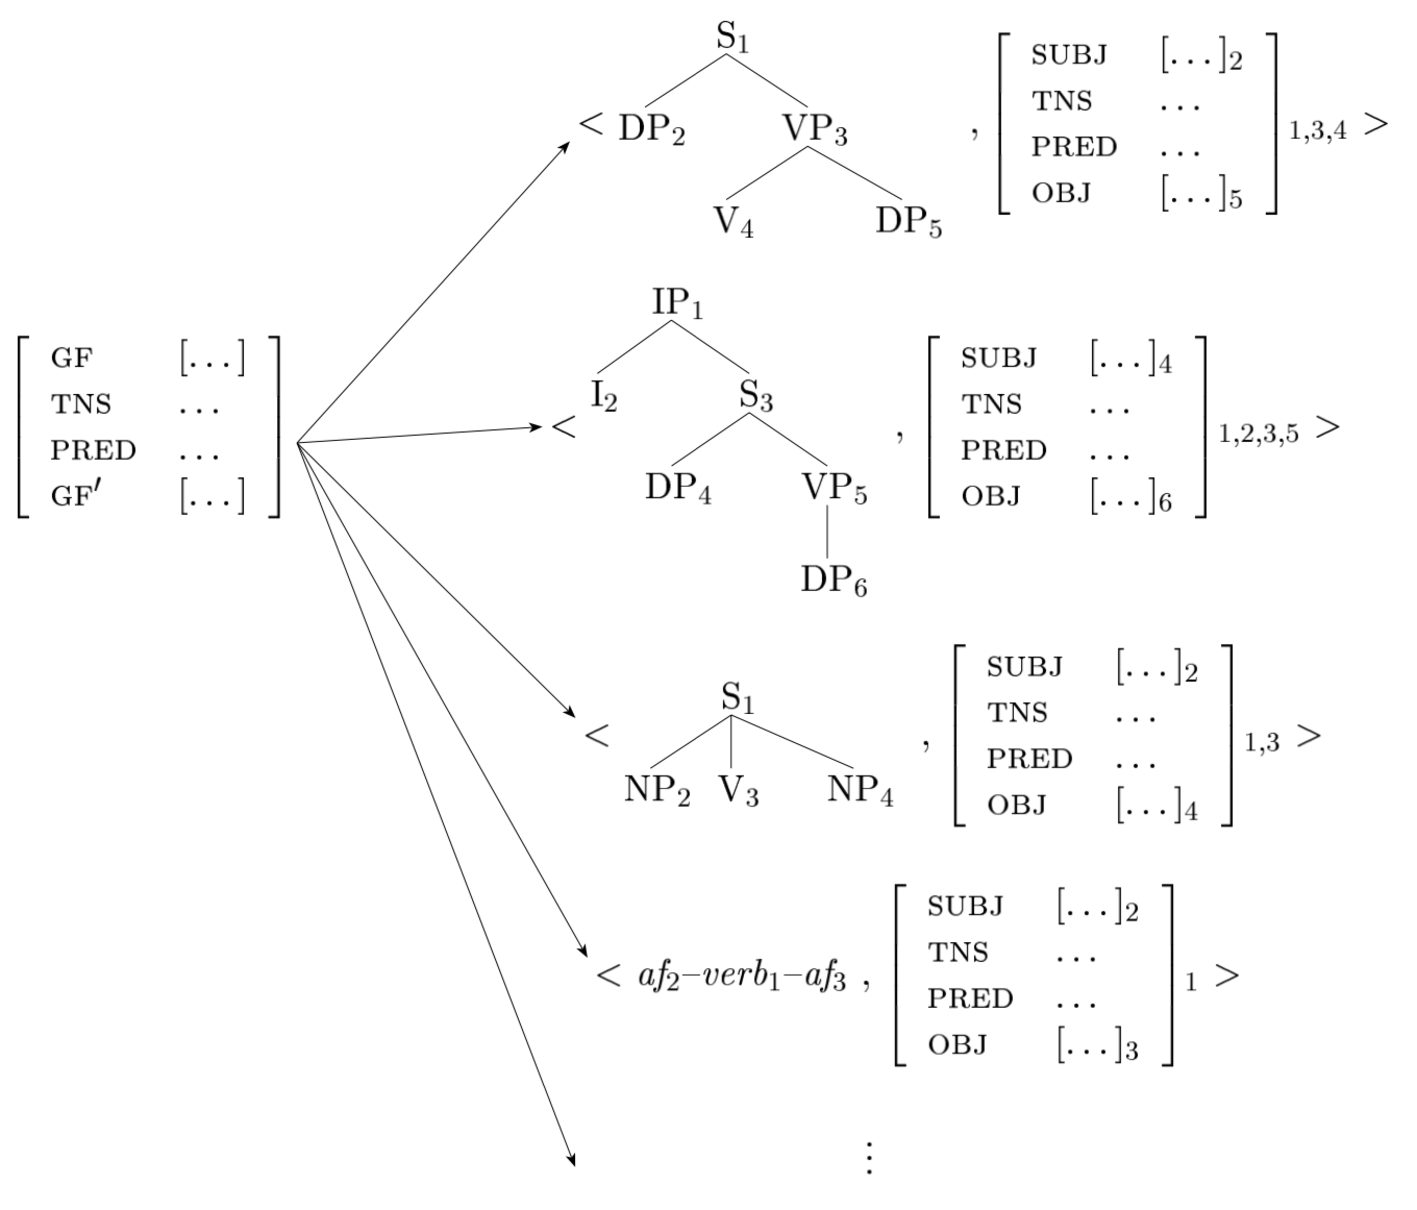
\includegraphics[scale=.45]{figures/OT/OT-candidate-generation.pdf}
\caption{Illustration of candidate generation in OT-LFG \citep{Bresnan-Explaining-Morphosyntactic}: an underspecified functional structure (on the left) is the basis for generating full LFG analyses (c-structure/f-structure pairs) whose f-structure is subsumed by the input.}
\label{fig:OT-LFG-Gen}
\end{figure}


Early work on OT syntax sometimes % ?? more precise?
relied on an intuitive and informal conception of the syntactic structures that should compete with each other in the same candidate set.
To preserve the idea from OT phonology that all conceivable alternatives for saying the same thing are included in the candidate set, the natural assumption for the input in OT syntax is an abstract representation of the syntactically relevant \emph{semantic content} of an utterance. As \citet{Bresnan-96-LFG-conference} points out, this intuition can be cashed out straightforwardly if candidate generation is based on a monotonic unification formalism like LFG: the input can be operationalized as a partial representation including the relevant semantic information, and the set of candidates as all the complete representations expanding this input representation -- in the case of LFG pairs of c-structures and corresponding f-structures that are subsumed by the input presentation, as is illustrated in \figref{fig:OT-LFG-Gen} from \citet[]{Bresnan-Explaining-Morphosyntactic}. Cross-linguistic variation at the level of constituent structure is captured by including all typologically different options for expressing some core semantic information in the candidate set. 

\newpage

A formal definition for the candidate generation function \emph{Gen} in OT-LFG is shown in (\ref{ex:Gen-def}) \citep[][74]{Kuhn-CSLI-book}.\footnote{The language $L(G)$ generated by an LFG grammar $G$ is here defined as the set of tuples $\langle T, \Phi\rangle$ such that $T$ is a c-structure generated by the context-free skeleton in $G$ and $\Phi$ is a valid f-structure for $T$ according to the functional descriptions in $G$. } 
\emph{Gen} depends on an LFG-type base grammar $G_{\emph{inviol}}$, which specifies the space of structurally valid candidate tuples from the full typological spectrum by means of the `inviolable principles', and is applied to a partially specified f-structure $\Phi_{\emph{in}}$.

\ea\label{ex:Gen-def}
Restricted definition of \emph{Gen}\\
\setlength{\tabcolsep}{3pt}
\begin{tabular}[t]{lllll}
 $\emph{Gen}_{G_{\emph{inviol}}}(\Phi_{\emph{in}})$ & = & \{ & $\langle T, \Phi'\rangle\in L(G_{\emph{inviol}}) \, |  \, \Phi_{\emph{in}} \sqsubseteq \Phi'$, where $\Phi'$ contains  &  \\
  & & & no more semantic information than $\Phi_{\emph{in}}$ & \} \\
\end{tabular}
\z


\noindent
The candidate set generated by \emph{Gen} includes all c-structure/f-structure pairs from the base grammar whose f-structure $\Phi'$ (i) is subsumed by the input f-structure $\Phi_{\emph{in}}$ and (ii) does not add any semantic information.\footnote{The restriction excluding surplus semantic information will be addressed in \sectref{sec:OT:comp-considerations}.}

The violable constraints in OT-LFG operate on the candidate representations. It is in principle conceivable to include the detection of constraint violations already in the specification of the base grammar $G_{\emph{inviol}}$, using disjunctive f-annota\-tions of the kind shown in \sectref{sec:OT:OT-style-initial-example} on soft constraints in computational grammar development and introducing marks to a special $o$-projection for counting. However, the specification would presumably become unmanageable fast, since the representational patterns addressed in the various constraints are interdependent; moreover, many constraints address not only patterns in f-structures, but make reference to portions of c-structure. The formalization of OT constraints in \citet[][ch.~4]{Kuhn-CSLI-book} therefore proposes to leave constraint marking out of $G_{\emph{inviol}}$ and assume a conceptually separate step for detecting the constraint violations for each c-structure/f-structure pair in the candidate set. This step can employ straightforward descriptive constraint \emph{schemata} which use a special metavariable $\star$ that is successively being instantiated to every structural element in a candidate analysis, i.e., to each c-structure node, and to each (sub) f-structure.

In (\ref{ex:constr-formal}), the schema-based formal capturing of Bresnan's (\citeyear{bresnan00opt}) constraints \textsc{Op-Spec} and \textsc{Ob-Hd}, which were discussed in \sectref{sec:OT:initial-example}, is seen \citep[for details, see][90ff]{Kuhn-CSLI-book}:\footnote{The schemata assume appropriately defined auxiliary predicates \emph{cat} (for category) etc.}

\ea\label{ex:constr-formal}
\ea
\textsc{Op-Spec} (`An operator must be the value of a \textsc{df} in the f-structure.')

\ \ \begin{tabular}[t]{l}
$(\emph{f-str}(\star) \wedge \exists v.[(\star \, \textsc{op})=v])$\\ $\rightarrow \exists f.[(f \, \textsc{df})=\star]$
\end{tabular}

``If $\star$ is an f-structure bearing a feature \textsc{op} (with some value $v$), then there is some f-structure $f$ such that $\star$ is embedded in $f$ under a \textsc{df} function.'' 
\ex \textsc{Ob-Hd} (`Every projected category has a lexically filled extended head.')


\ \ \begin{tabular}[t]{l}
$(\emph{cat}(\star) \wedge (\emph{bar-level}(\star,1) \vee \emph{bar-level}(\star,2))$ \\ $\rightarrow \exists n.[\emph{ext-hd}(n,\star)]$
\end{tabular}

``If $\star$ is an X-bar or X-max category, then there is some node $n$ which is the extended head of $\star$.''
\z
\z

\noindent
The evaluation function \emph{Eval} is operationalized as a trial of all schemata in the constraint set $\cal{C}$ on every structural element of a candidate analysis (c-structure node or partial f-structure).
For the trial, the metavariable $\star$ is instantiated to the element under consideration; the count for the relevant constraint is increased in case the proposition is satisfied. The language-specific ranking $\gg_{\cal{L}}$ over the constraints then controls the filtering of the most harmonic candidate(s), in the same way as illustrated in  \figref{fig:tableau1} in \sectref{sec:OT:initial-example}.


All candidates that are optimal (under the constraint ranking for a given language ${\cal L}$) for some underlying partial f-structure $\Phi_{\emph{in}}$ then form the language (= set of c-structure/f-structure pairs) generated by an OT-LFG system for language ${\cal L}$ \citep[][117]{Kuhn-CSLI-book}:

\ea\label{ex:OT-Lang-def}
Definition of the language generated by an OT-LFG system ${\cal O} = \langle G_{\emph{inviol}},\langle{\cal C},\gg_{\cal{L}}\rangle\rangle$ for language ${\cal L}$:

\setlength{\tabcolsep}{3pt}
\begin{tabular}[t]{lllll}
 $L(\cal{O})$ & = & \{ & $\langle T_j, \Phi_j\rangle\in L(G_{\emph{inviol}}) \, | $\\
  & & & $\, \exists \Phi_{\emph{in}}: \langle T_j, \Phi_j\rangle\in \emph{Eval}_{\langle\cal{C},\gg_{\cal{L}}\rangle}(\emph{Gen}_{G_{\emph{inviol}}}(\Phi_{\emph{in}}))$ & \} \\
\end{tabular}
\z

The OT-LFG formalization thus provides a declarative, fully operationalized  framework for specifying a theory of the typological space of options for a range of grammatical phenomena, predicting specific realization patterns for languages associated with certain constraint rankings.
Computational considerations, in particular regarding the complexity of \emph{Gen}, will be addressed in \sectref{sec:OT:comp-considerations}.


Combining the OT concept of competition-based specification of grammatical knowledge with the LFG formalism for operationalizing the components of such an account was beneficial for both sides: For OT theorists interested in exploring the expressiveness of the Optimality-Theoretic approach when applied to phenomena from the broad field of morphology/syntax/semantics, the OT-LFG framework provided a basis whose formal and computational properties were well understood. Consequently, (i) concrete accounts for phenomena of interest could be worked out and tested against attested linguistic data, and (ii) formal and computational implications of the novel conceptualization of modeling grammatical knowledge could be pinpointed. In the reverse direction, the LFG community benefited from the extension of the classical formalism, since OT-LFG provided a formalized framework for predicting patterns in the variation observed across languages (and within a language). By couching an LFG account for a phenomenon in the OT-LFG framework, its generality thus becomes testable against empirical data from language typology. And even when trying to capture variation patterns within a single language, an OT-LFG approach readily supports a reasoning that reduces the range of available realization options to a small set of independently justifiable directives.

\subsection{OT-LFG's conceptual advantages over a derivational base formalism}
\label{sec:OT:advantages-over-derivational-base-formalism}

A large proportion of work in OT syntax is not couched in the OT-LFG framework, but assumes a derivational base formalism such as Principle-and-Parameter Theory \citep{chomsky1981lectures} or Minimalism % ?? citation
(see Grimshaw's \citeyear{Grimshaw97} original account and much subsequent work, e.g., \citealt{Pesetsky98}). % ?? some more
With candidate analyses that are inherently derivational, 
an implementation of the original OT idea -- that the input corresponds to the semantic content of the expressions under consideration --
inevitably leads to a more complicated architecture.
In the study of syntax, the expressions under consideration are full sentences; so, to implement the original OT idea, all alternative surface sentences  expressing the same semantic content should be included in a candidate set. The complication for an OT architecture now arises from the fact that 
in a Chomskyan derivational approach, semantic interpretation is located at the level of logical form (LF), which is by definition one of the end points of a derivational process that starts out from a D-structure (as in the T-model underlying Principle-and-Parameter Theory, shown in \figref{fig:T-model}) or a set of lexical items, the ``numeration''. %\todo{Have a figure with the Y-shaped process}


\begin{figure}[ht]
    \centering
    \begin{tabular}{cccccccc}
     & \multicolumn{5}{c}{\fbox{lexicon, X-bar theory}} & \\
     & & \ \ \ \ \ \ \ & $\downarrow$ & \ \ \ \ \ \ \ \ & \\[.5ex]
     & \multicolumn{5}{c}{D-Structure} & \\[.5ex]
     &  & & $\downarrow$  &  \multicolumn{3}{l}{\fbox{\rule[0mm]{0mm}{1.8ex} move $\alpha$}}  \\[.5ex]
     & \multicolumn{5}{c}{S-Structure} & \\[.5ex]
& \fbox{spellout}  &  & & & \fbox{\rule[0mm]{0mm}{1.8ex} move $\alpha$}  & & \\[.5ex]
  & & $\swarrow$ & & $\searrow$ &    \\[.5ex]

\multicolumn{2}{c}{PF}  & & & & LF \\
\multicolumn{2}{c}{(phonological} & & &  & (logical \\
\multicolumn{2}{c}{form)}  & & & & form) \\
     \end{tabular}
     \caption{The T-model (or Y-model) of the derivation processes underlying a single analysis couched in Principle-and-Parameter Theory \citep{chomsky1981lectures}}
\label{fig:T-model}
\end{figure}


In a non-OT framework, the derivational processes that lead to a phonological form and a logical form are controlled by language-particular factors. When the derivational processes are taken to be the candidates of an OT system that adheres to the richness of the base, the derivational mechanisms have to be opened up in such a way that all language-particular restrictions on the derivations are lifted -- generating all conceivable variants as alternative candidate derivations and leaving the calculation of language-particular effects to \emph{Eval}, which selects the optimal derivation based on the constraint ranking. The input (for the definition of the OT candidate set) has to be (some relevant part of) an LF representation, and the set of candidates that \emph{Gen} assigns to such an ``input'' LF must be all derivations that \emph{end in} this LF via unconstrained derivation -- from any possible starting point (i.e., any numeration of lexical items that could arrive at this LF through unconstrained transformational derivations). Leaving aside concerns regarding the computational tractability of such a system, it is challenging to conceptualize the workings of the OT constraints if the candidate-internal derivation is taken literally as a (potentially destructive) structure-transforming process: if the evaluation of candidate derivations does not take place until a particular LF has been reached, how can the constraints be used to control the language-specific choices in the derivation steps happening early on in the process?  

The constraint evaluation challenge can be resolved by viewing the derivational process inherent to the candidates as some abstract process that produces a \emph{representation} including a record of all relevant steps (such as traces of a movement). With this representational strategy, a definition of the candidate set via a shared LF becomes possible. Let us call this an LF-as-input OT system, which preserves the original, meaning-related concept of the OT input (but enforces an abstract view of the derivations, with a representational record).

For a research approach starting out with a derivational framework, it may seem more natural however to resolve the constraint evaluation challenge in a different way: giving up the fully meaning-related notion of the OT input, one can turn to a different way of characterizing the set of competing candidates: since the derivations have their own technical starting point -- D-structure or a numeration of lexical items -- 
why not adopt a conceptualization in which this part of the candidate derivations constitutes 
the input for the OT system and have \emph{Eval} compare the various possible derivations with identical D-structures/nu\-mer\-a\-tions? Important typological considerations regarding syntax and morphology \emph{can} be addressed under this view.
In fact, when a study focuses on a small set of specific phenomena -- as is common practice both for typological and for language-particular studies in linguistics -- the two approaches are often indistinguishable, since the (supposedly) \emph{relevant} variation across candidates on which the study is centered originates from the same derivational subprocess across all candidates.
This is presumably the explanation for the fact that
the simpler system is often tacitly assumed. However, in situations where attention is not focused on a narrowly delineated range of phenomena, the two ways of conceptualizing the input \emph{do} make an enormous difference. Only a semantically based input will leave the choice among realizations that differ in the lexical material in non-trivial ways to \emph{Con} and \emph{Eval}.\footnote{Of course, not all accounts incorporating a competition-based subprocess are necessarily following the idea that all cross-lingual variation should be reduced to a global, fully meaning-based optimization. It is also conceivable to construe distinct derivational steps as separate, self-contained optimizations (compare e.g., \citealt{HeckMueller2000,Mueller2003}).  Many approaches explicitly couched in a derivational setting indeed assume fairly restricted structural or derivational \emph{domains} of local optimization \citep[sec.~4]{GMueller2012}.  %\todo{check Mueller REF!} . % Heck/Mueller 2000, Mueller 2002, Heck et al. ?? cite work on cyclical application of OT
}  %\footnote{Also, a bidirectional optimization approach .... section .... only compatible with semantically based input ...} ?? 

A numeration-as-input approach generally imposes restrictions on the candidate space that are tied to particular languages (since semantically equivalent paraphrases of the same content which use different lexical material do not compete in the same candidate set). 
It is actually a consequence of the predominance of the numeration-as-input approach (and similar input conceptualizations) that \emph{language-particular ineffability} was considered a central issue for OT accounts of syntax. The issue can be characterized as follows: since by definition there is always a most harmonic candidate in any given candidate set, the OT approach appears to systematically exclude the possibility that in some languages there is no grammatical realization at all for a conceivable linguistic construction.
\citet{FanselowFery} provide the example in (\ref{ex:ineff}). While (\ref{ex:ineff}a) is grammatical in English, there is no grammatical way of saying (the equivalent of)  (\ref{ex:ineff}b). They argue that a standard system of OT syntax as Grimshaw's (\citeyear{Grimshaw97}) will include a candidate set of alternative clause realizations for (\ref{ex:ineff}b), and one of them will inevitably be the most harmonic, incorrectly predicting that there is some grammatical realization used this set of lexical items.

\ea\label{ex:ineff}
  \ea Who did the president think that the foreign minister met in Afghanistan?
  \ex[*]{ Who did the president resign although the foreign minister met in Afghanistan? }
  \z
\z

\noindent
Note however that with a sufficiently abstract semantic input, an LF-as-input OT system \emph{could} be devised that makes reasonable predictions for all languages: Where there is no compact realization of a thought in a single clause, a more verbose, multi-clause paraphrase can be used (for (\ref{ex:ineff}b) maybe \emph{Who was it that the foreign minister met in Afghanistan when the president resigned nevertheless?}). This appears like a plausible analogy to examples from phonology, where some languages enforce a very unfaithful realization of loan words or foreign names that fall outside the phonological patterns of a language (as exemplified by (\ref{ex:plan}) above). Thus, the  language-particular ineffability problem arising in numeration-as-input approaches is not a problem under a global meaning-based conceptualization of the input.

The considerations in this subsection have shown that while a competition-based construal of dedicated derivational subprocesses may be fruitful in order to systematically derive typological patters for a certain submodule of a broader derivational theory of grammar, the original OT idea of deriving all cross-lingual differences -- and thus learnability -- as an effect of constraint reranking presupposes a comprehensive global competition among all alternative candidate expressions for a given underlying meaning. For capturing constraint evaluation in global competition with a derivational base formalism, there does not seem to be a good alternative to using representational traces of the (abstract) derivational process inherent to each candidate representation. 

Bresnan's (\citeyear{Bresnan-96-LFG-conference}) recasting of Grimshaw's (\citeyear{Grimshaw97}) account of extended projections -- employing Extended Head Theory as sketched in \sectref{sec:OT:intro} -- can be viewed as a blueprint of a strategy that translates some relevant key aspects of a derivational approach into a representational approach. So, one can effectively view OT-LFG not only as an OT extension of the LFG framework; it also provides a feasible implementation for LF-as-input approaches, in particular a whole range of work that follows the general spirit of Grimshaw's (\citeyear{Grimshaw97}) proposal. %\todo{Samek-Lodovici, Vikner !?} % ?? list of examples

To sum up the previous and this section, OT-LFG as proposed by \citet{Bresnan-96-LFG-conference,bresnan00opt,Bresnan-Explaining-Morphosyntactic,Bresnan-Lexicon-in-OT} spells out a conceptualization of OT syntax that allows for a clean and comprehensive separation of language-independent candidate generation and violable constraints capturing the spectrum of typological variation. LFG's representational framework makes this separation conceptually simple. Global competition, for instance between morphological vs.\ syntactic means of expressing for realizing an underlying feature is naturally accounted for since LFG assumes parallel correspondence among all representational structures. 


\subsection{OT-LFG: Computational considerations}
\label{sec:OT:comp-considerations}

Conceptually straightforward as it is, the idea of relying on feature structure subsumption to define the set of candidate analyses (i.e., tuples of c-structure, fully specified f-structure and potentially more LFG projections) in \emph{Gen} as specified in \sectref{sec:OT:OT-Syntax} raised computational concerns. \citet{Johnson98} points to the issue that the parsing problem for an OT-LFG grammar is undecidable in the general case. To solve the parsing problem given a string $s$, all optimal analyses have to be found that have $s$ as the yield of their c-structure tree.\footnote{\citet{Johnson98} assumes stronger conditions for the optimal candidate: the input representation determined in the first step needs to be included in the optimal analysis of the string. This corresponds to (strong) bidirectional optimality, as discussed in \sectref{sec:OT:biOT}. For standard OT, only the production-based competition is relevant, as assumed in the remainder of this section.} % DONE: Point out that this is a variant of Johnson's construction (he makes the argument with a bidirection optimization assumption


\begin{figure}[ht]
    \centering
    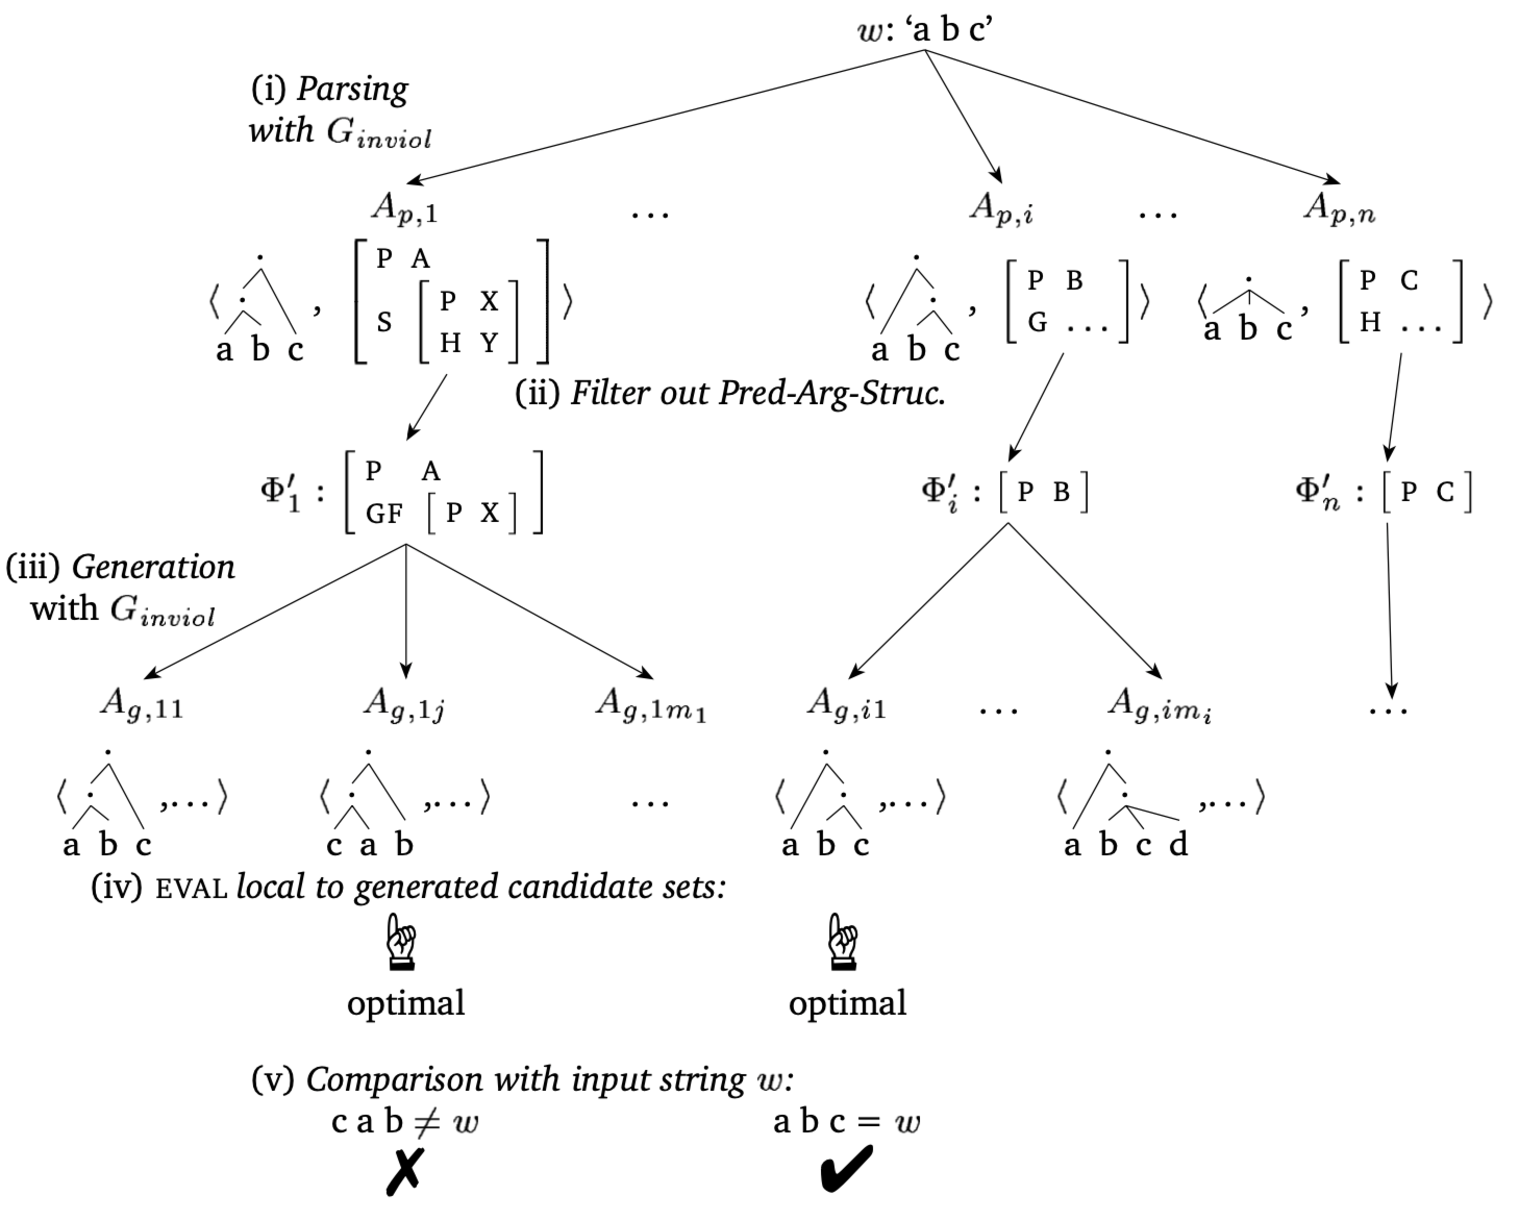
\includegraphics[scale=.45]{figures/OT/OT-parsing-figure.pdf}
\caption{Illustration from \citet[173]{Kuhn-CSLI-book} for the parsing procedure for a standard OT system, with grammaticality based on production-based optimality.}
\label{fig:OT-parsing}
\end{figure}


\figref{fig:OT-parsing} from \citet[173]{Kuhn-CSLI-book} illustrates the procedure with a semi-ab\-stract example.
In a first step
(i) all potentially underlying input representations have to be found. This can be achieved by standard LFG parsing (which is decidable), using the base grammar that defines the set of all universally available candidate structures. The input information is by definition part of the f-structure in each candidate. This predicate-argument structure representation has to be filtered out
(step (ii)). In a next step
(iii), for each potential underlying input representation, the set of all candidates has to be generated (including the original as well as all alternative full c-structure/f-structure tuples); the constraints are applied to each candidate
(iv) and the most harmonic candidate can be determined, given the relevant constraint ranking. This candidate is only included in the set of valid analyses for the original string $s$ if $s$ is indeed the yield of the optimal candidate (v).

We note that step (iii) involves generation with an LFG-type grammar from a partially specified f-structure. \citet{Wedekind99} shows that the general problem of generation from partial f-structures, given some LFG grammar, is undecidable. This implies that there could be cases in which the candidate set for a given input f-structure cannot be computed, so it would also be impossible to determine the effect of an OT system. However, Wedekind also points out that the decidability problem for generation with plain LFGs occurs only with certain technical feature representations that are not used to represent the semantics of natural-language sentences. How does this translate to the application of an LFG-style grammar in OT candidate generation? Is it possible to formulate restrictions on admissible partial f-structures and thus guarantee decidability of the parsing problem?

Potentially problematic cases are candidates that include violations of faithfulness constraints, as they are for instance assumed to derive \emph{do}-insertion in English questions \citep[ex.~44]{bresnan00opt}.  As we will see in the following, restrictions on the formalism can be devised that guarantee decidability but nevertheless permit the use of faithfulness constraints to derive syntactic variation of this kind.
Taking advantage of the explanatory potential of OT, Bresnan's (\citeyear{bresnan00opt}) analysis does not stipulate a special, \textsc{pred}-less lexicon entry in \emph{do} insertion (like in standard LFG), but derives insertion of an additional verb as a consequence of the ranking of violable constraints.
To achieve this effect, the \emph{Gen} function underlying in this system has to be able to add ``unfaithful material'' quite freely. Does this mean that we are confronted with the decidability problem?

\newpage
As \citet[ch.~4]{Kuhn-CSLI-book} discusses, the option of adding unlimited amounts of material in a candidate is not only undesirable from a computational point of view. It also goes against the key idea of treating all candidates as potential verbalizations of some identifiable semantic content. The definition of \emph{Gen} should therefore be restricted in such a way that the candidates' f-structures (i.e., the interpretable part of the representation) are not only subsumed by the input f-structure, they also may not contain any additional semantic information.\footnote{It is allowed for candidates to contain additional non-semantic f-structure information and material at the level of c-structure and other projections; this is unproblematic for decidability, since the amount of information that can be added is bounded by the size of the grammar.} With this restriction, it can be guaranteed that the set of candidates stays computationally tractable (\citealt{kuhn-2002-ot}, \citealt[199ff]{Kuhn-CSLI-book}). The definition (\ref{ex:Gen-def}) above already incorporated the necessary restriction.

\begin{figure}[bh]
\vspace{-6em}
\begin{tabular}{ll}
\begin{tabular}{cl}
\\[10em]
\rnode{l1a}{$\left[\begin{array}{ll}
\textsc{pred} & \textrm{`do'} \\
  \end{array}\right]$} & \raisebox{-1.5ex}{$\lambda$}\\
  \\
\rnode{l1b}{$\left[\begin{array}{ll}
\textsc{tns} & \textsc{past} \\
  \end{array}\right]$} & $\lambda$\\[3ex]
  \\
\rnode{f}{$\left[\begin{array}{ll}
\textsc{pred} & \textrm{`say(x, y)'} \\
\textsc{subj} & [$ \textsc{pred} \ `\textsc{pro}'  $] \\
\textsc{obj} & [$ \textsc{pred} \ `\textsc{pro}' $] \\
\textsc{tns} & \textsc{past} \\
  \end{array}\right]$} & \raisebox{-1.5ex}{$\phi$} \\
  \\
  \rnode{l2}{$\left[\begin{array}{ll}
\textsc{pred} & \textrm{`say'} \\
  \end{array}\right]$} & $\lambda$ \\[1ex]
\end{tabular}
&
\raisebox{5em}{\begin{forest} 
[IP
  [NP [{she},roof] ]
  [I$'$
    [\rnode{I}{I} [did]]
    [VP [V$'$
        [\rnode{V}{V} [say] ]
        [NP [{that},roof] ]
        ]]]]
\end{forest}}
\end{tabular}
\nccurve[nodesepA=4pt,nodesepB=0pt,angleA={225},angleB={0},linewidth=.5pt,linestyle=dashed]{->}{I}{l1a}
\nccurve[nodesepA=4pt,nodesepB=0pt,angleA={225},angleB={0},linewidth=.5pt,linestyle=dashed]{->}{I}{l1b}
\nccurve[nodesepA=2pt,nodesepB=0pt,angleA={180},angleB={0},linewidth=.5pt,linestyle=dashed]{->}{V}{l2}
\nccurve[nodesepA=2pt,nodesepB=0pt,angleA={225},angleB={0},linewidth=.5pt]{->}{I}{f}


\caption{Illustration of a candidate incurring a faithfulness violation, following the technical formalization of \citet[112]{Kuhn-CSLI-book}; c-structure nodes project not only to f-structure (via function $\phi$), but also to a (very local) lexical structure (via function $\lambda$).} 
\label{fig:do-insertion}
\end{figure}


\figref{fig:do-insertion} illustrates a formalization of faithfulness violations that is compatible with this restriction and can be used to derive \emph{do} insertion in English. The key idea from \citet[ex.~44]{bresnan00opt} is that the lexical contribution of elements that are inserted ``unfaithfully'' (as a way of satisfying some other constraint that is higher-ranking than faithfulness) does not make it into the candidate's f-structure. The technical operationalization from \citet[112]{Kuhn-CSLI-book} uses a special $\lambda$-projection to keep track of all lexical contributions from the words, which may or may not re-appear in f-structure. In case they do \emph{not} re-appear, a violation of a faithfulness constraint (\textsc{Dep-IO}) will be recorded by \emph{Eval}.


The lexical entries underlying the analysis in \figref{fig:do-insertion} are specified as shown in (\ref{ex:lex-entries-did-say})  \citep[adapted from][ex.~140]{Kuhn-CSLI-book}: 

\ea\label{ex:lex-entries-did-say}
\catlexentry{did}{I}{$g_1 = \lambda({\mathcal M}*)$\\
  $(g_1 \, \textsc{pred}) = \textrm{`do'}$  \\
  $\{ \, g_1 = \, \uparrow \, \}   $\\
  $g_2 = \lambda({\mathcal M}*)$ \\ 
  $(g_2 \, \textsc{tns}) = \textsc{past}$  \\ 
  $\{  \, g_2 = \, \uparrow  \, \}  $}\\[1ex]
\catlexentry{say}{V}{$g_1 = \lambda({\mathcal M}*)$\\
  $(g_1 \, \textsc{pred}) = \textrm{`say'}$  \\
  $\{  \, g_1 = \, \uparrow  \, \} $}
\z

\noindent
In these entries, the functional annotations make use of local metavariables (such as $g_1$ and $g_2$) in the following way:
The equation $g_1 = \lambda({\mathcal M}*)$ defines $g_1$ as the variable name for an attribute-value structure that is $\lambda$-projected from the current element's c-structural mother (= the node I for \emph{did}). The equation $(g_1 \, \textsc{pred}) = \textrm{`do'}$ introduces a \textsc{pred} feature and value into the attribute-value structure. The third equation $\{ \, g_1 = \, \uparrow \, \}$ identifies the local l-structure with the c-structural elements normal f-structure (i.e., its $\phi$-projection; recall that $\uparrow$ is defined as ${\mathcal M}*$). What is crucial is that the third equation is enclosed in curly brackets, which means that it is applied optionally. Hence, the lexical specification will either be included in the f-structure or not. (Since the rest of the LFG structure leads to an identification of the f-structure projected from \emph{did} and from \emph{say}, maximally one of the two entries can introduce their \textsc{pred} value to f-structure.)

The enormous variation opened up by this optionality is controlled by the faithfulness constraint \textsc{Dep-IO}, which in this setup can be formalized as in (\ref{ex:Dep-IO-formal}):

\ea\label{ex:Dep-IO-formal}
\textsc{Dep-IO} (referred to as \textsc{Fill} in early OT work)\\
General OT formulation \citep[][68]{kager99}: `Output segments must have input correspondents.'

\ \ \begin{tabular}{l}
$(\emph{atomic-f-str}(\star) \rightarrow$\\ $\forall n, P.[ ( \emph{cat}(n) \wedge \emph{feature-path}(P) \wedge (\lambda(n) P)=\star ) \rightarrow (\phi(n) P)=\star] )$
\end{tabular}

``For all categories $n$ and feature paths $P$, if $\star$ is an atomic value under $P$ in the $\lambda$-projection from $n$, then $\star$ is also the value under  $P$ in the $\phi$-projection from $n$.'' 
\z

\noindent
Recall that in the application of the \emph{Eval} function, every structural element in a candidate representation -- i.e., every c-structure node, every local f-structure, and also every local l-structure -- will be tested for all constraints. For the topmost l-structure seen in \figref{fig:do-insertion}, $\star$ will be instantiated to the \textsc{pred}-value `do', which \emph{is} an atomic f-structure and which is also in the $\lambda$-projection of a node $n$ (namely I) under a path $p$ (namely \textsc{pred}). So to satisfy the \textsc{Dep-IO} faithfulness constraint, \textsc{pred} `do' should also be in the f-structure for I, which it is not. This leads to the desired effect of capturing an insertion in c-structure which has no correspondence in f-structure as a \textsc{Dep-IO} violation.

To sum up, the insertions that are required to implement a generalized OT account are compatible with the restricted definition of \emph{Gen}. By definition, the semantic information in a candidate's f-structure is always the same as the semantic information in the underspecified input f-structure $\Phi_\emph{in}$. Additional material can only occur in locally projected l-structures. While it is not forbidden to have infinitely many distinct candidate structures for an input f-structure, the restriction keeps the candidate set computationally tractable \citep[][ch.~6]{Kuhn-CSLI-book}.\footnote{Exploiting results from \citet{kaplan-wedekind-2000-coling}, recursive loops that lead to infinite candidate sets can be captured in a tractable way.}



\subsection{Excursion: The cognitive status of ``directional'' candidate set specification}
\label{sec:OT:psycho-real}

As established in the previous subsection, it is possible to provide
a declarative formal characterization of the language generated by an OT system. Thanks to the non-derivational character of (tuples of) LFG structures, it is possible to use the sharing of the semantic part of the structures as the defining element for candidate sets (independent of the question of how a computational system might be implemented that takes a string of words as an input and produces all fully specified LFG structure tuples with that surface string that are optimal for some input according to the OT system for a given language). Moreover, it can be shown that the task of determining whether a string of words is in the language generated by an OT system is not computationally undecidable.
This subsection is an excursion that discusses a reaction that LFG practitioners might have when confronted with the multi-step breakdown of the abstract parsing task for an (LFG-based) OT system sketched in \figref{fig:OT-parsing}: the assumption of a back and forth of generation and parsing processes seems to go against the goal of developing a cognitively plausible model architecture to capture grammatical knowledge. 

The intuitive algorithmic breakdown of parsing with plain LFG does not carry over to parsing in the OT-LFG framework, which necessarily has to incorporate a production-based directionality, while parsing models comprehension.  Parsing with a plain LFG grammar follows the logic of the structure specification step by step: given a string, matching lexicon entries and c-structure rewrite rules are used to construct a set of c-structure trees spanning the string. To narrow the set down to the trees which correspond to a valid f-structure, functional descriptions from the lexical annotations and the rule annotations are then taken into account in a process of model construction (in a feature logic), and wherever we find a valid f-structure, we have one possible analysis for the input string. The intuitive simplicity of the algorithmic breakdown has presumably played a role in the attraction of the LFG formalism as a psychologically realistic framework -- in particular as it contrasted with the model of Chomskyan derivational approaches, which work with a notion of an underlying deep structure (D-structure or numeration). The theoretically motivated transformation of an underlying deep structure into a surface structure does capture intuitions regarding the highly systematic relationship between expressions like \emph{the cat drinks milk} and \emph{what does the cat drink?} or between \emph{she saw the cat} and \emph{the cat was seen}.  But in comprehension, a listener is confronted with the linear string from a surface structure (say, \emph{the cat was seen}), and there is no cognitively intuitive algorithmic process that leads back to conceivable underlying deep structures. When spelling out a parsing procedure with OT-LFG, we now find ourselves in a similar situation: if we translate the bidirectional characterization of the set of valid structures for a given string into an algorithmic procedure, we do not arrive at a plausible rendition of what could be going on in comprehension. %\todo{check this subsection for redundancies and lengthiness} 

One might suspect that these considerations challenge the cognitive plausibility of Optimality Theory. It should be noted however that there is an oversimplification in the reasoning that assumes a direct conceptual mapping of a declarative specification of some function (such as the function from a string of words to a set of c-structures associated with valid f-structures) to the seemingly straightforward algorithmic breakdown of this function.
It is misleading in the general case to assume that an intuitively appealing translation of a composite function into some procedure is the only option for realizing the theoretically motivated function in a cognitive system. As a matter of fact, there would be no computationally tractable parsers for standard LFG if one relied on the simple-most translation of the conceptual steps underlying grammatical specification in LFG into an algorithm. 
As the discussion in \citet{maxwellkaplan96} illustrates, LFG parsing performs a highly sophisticated interleaving of the various sources of grammatical and lexical knowledge. Vice versa, Edward Stabler's work on the formalization of Chomskyan derivational grammar models (e.g., \citealt{Stabler2011,Stabler2013}) shows that algorithmic solutions do not have to stick to the seemingly counterintuitive procedures in the underlying theoretical characterization. %\todo{rewrite next paragraph a little} 

The complicated procedural breakdown of the parsing task for OT systems follows in fact from the decision to incorporate an important consideration into the conceptualization of grammatical knowledge that has nothing to do with the procedural knowledge needed for parsing a particular given input string, but rather reflects a language learner's and adult speaker's conscious or tacit knowledge of the expressive \emph{potential} that lies in the language system: for a speaker of language X to know the grammatical way of expressing something in X amounts to knowing which other potential ways of expressing the same thing are not available in X.\footnote{When working with a classical grammar formalism, the formal model of a speaker's grammatical knowledge provides no way of making this differential knowledge explicit, yet to arrive at a particular formal grammar in language acquisition, the learner must have pruned away certain realization options that the language under consideration does not exploit.} During the acquisition of X, the speaker will have learned from exposure to adult speakers' language behavior which realizational variants can be completely excluded. So, the adult speaker's grammatical knowledge may well be thought of computationally as a ``hard-wired'' input-output mapping that freezes the patterns which have stabilized in the competition system (superseding a dynamic acquisition phase, during which the relevant constraint rerankings were triggered for language learner).

As a side note, the ``pre-compilation'' of a cascade of optimality constraints with their step-by-step filtering effect into a single input-output function was subject to research in the context of OT systems that can be fully formalized with finite-state systems. \citet{karttunen-1998-proper} proposed a special finite-state operator (so-called lenient composition) that has the effect of turning a sequence of individual constraints formulated as transducers into a single transducer with the same effect as an OT competition.\footnote{A similar approach is discussed by \citet{FrankSatta98}.} To achieve a similar computational effect for a syntactic OT-LFG system, the internal data structures built up during parsing (following a chart-based or dynamic programming approach) would have to be re-designed to simultaneously incorporate a production-based and a comprehension-based directionality -- which could then be instantiated in a single bottom-up algorithmic pass, avoiding direct bidirectionality processing (compare the ``interleaved'' bidirectional processing approach proposed in \citealt{Kuhn-ACL2000}).
Since work in computational linguistics focusing on learning without any language-specific prior knowledge had already reached a relatively advanced state using different approaches, there was no substantial practical interest in putting the full OT-LFG account to use on a larger scale. 

\subsection{OT-style constraint ranking in broad-coverage grammars} 
\label{sec:OT:OT-style-ranking}

\sectref{sec:OT:OT-style-initial-example} provided an illustration of the constraint ranking mechanism implemented in the XLE system, which is widely used in grammar development. The examples showed how violable constraints allow grammar writers to include rule variants for infrequently occurring constructions without causing a proliferation of implausible readings for canonical constructions.\footnote{Computationally, we can note in the light of \sectref{sec:OT:comp-considerations} that XLE's OT-style constraint ranking is not normally used to modify the notion of grammaticality from the base grammar; hence, the additional complexity of a two-way application of the grammar in parsing and generation mode does not arise.}

The XLE implementation of violable constraints via a special $o$-projection provides some further mechanisms that are of high practical value in broad-coverage grammar development.
The specification of the ranking of the optimality marks in (\ref{ex:optimality-order-extended}) illustrates some of these mechanisms. We will shortly go through a number of details, but first of all we note that the ranking is specified in the configuration section of the grammar code. This means that the relative ranking of the marks (and hence of the soft constraints) can be adjusted for different application scenarios of the grammar without changing the grammar code itself. Thus the ranking specification can be used to flexibly adjust the grammar to peculiarities of certain language registers or text domains.

\ea\label{ex:optimality-order-extended}
OPTIMALITYORDER \textsc{+PPasOBL (UnderstoodObj  TypeCoercionToTimeNoun) NOGOOD Missing3SgMarking STOPPOINT Fragment}.
\z

\noindent
In (\ref{ex:optimality-order-extended}), the highest-ranking mark  \textsc{PPasOBL} is preceded by a plus sign. This indicates that in the filtering of analyses, the mark is not considered to be negative, but positive. 
When the available readings differ in the count of \textsc{PPasOBL}, the ones with the \emph{maximal} number of marks survive. This provides grammar writers with a way of giving preference to a certain variant rather than having to ``punish'' a different variant, 
which, depending on the feature representation adopted, may be impractical. Rule (\ref{ex:VP2}) exemplifies the introduction of \textsc{PPasOBL} as a preference mark for the oblique object analysis of PPs (like in \emph{wait for someone}). The oblique reading will be preferred over the alternative of analyzing the PP as an adjunct whenever both are available. This has the effect of reducing the number of parses for a considerable number of input sentences.  In real-world uses of grammars, the available information makes it often hard to make an informed decision. So, in many application scenarios, it may be preferrable to make a (more or less arbitrary) decision in favor of one of the variants.\footnote{Contrary to the situation with very infrequent constructions that were discussed in \sectref{sec:OT:OT-style-initial-example}, the filtering may here have the effect that a contextually inappropriate analysis is chosen over the more appropriate analysis (for instance in \emph{Sue was waiting for hours}). But in a range of applications this may not be too problematic, while a reduction of the sources of ambiguity can be extremely helpful during the process of extending the grammar or fixing a certain problem. When the grammar is used in application scenarios in which it can be harmful to occasionally choose the contextually inappropriate variant, the preference mark can simply be taken out of the ranking specification, so the parser outputs both variants.} %\todo{make sure it is clear what is meant by ``informed decision''}

\ea \label{ex:VP2}
\phraserule{VP}{\rulenode{V\\\UP=\DOWN}
  \optrulenode{NP\\(\UP\OBJ)=\DOWN}
  \rulenode{PP*\\\begin{tabular}{lcr}\{&\DOWN$\in$ (\UP\ADJ)\\$|$&(\UP\OBLTHETA)=\DOWN\\&PPasOBL $\in$ $o$(*) & \}\end{tabular}}}
\z

The ranking in (\ref{ex:optimality-order-extended}) also illustrates the workings of parentheses and of some specially defined keywords. The marks \textsc{UnderstoodObj} and \textsc{TypeCoercionToTimeNoun}, which were introduced in \sectref{sec:OT:OT-style-initial-example}, are now jointly enclosed in parentheses to treat them as equally ranked. In grammar writing practice, such constraint ties are frequently used for phenomena that are independent from each other, since there is no grammar-internal justification for giving preference to one of them. %We will come back to the disambiguation decisions that are left undecided by the constraint tie strategy at the end of this section.

To the right of the two we see the mark NOGOOD. This is a predefined keyword that has the effect that all marks that follow receive a special interpretation that is best explained with a concrete example.
Consider \textsc{Missing3SgMarking}: this mark is introduced in the definition of the template \textsc{SubjNon3SgAgr} in (\ref{ex:agr-template}). This template is used in pres\-ent tense verb forms of English like \emph{I laugh} or \emph{they laugh}. There is a similar template for third-person singular forms like \emph{she laughs}. The third disjunct in (\ref{ex:agr-template}) covers the use of the form \emph{laugh} with a third-person singular NP like in *\emph{she laugh}, which is ungrammatical in standard English.  By providing this option, the grammar will robustly cover agreement mistakes or it can be used for varieties of English that include this variant.

\ea \label{ex:agr-template}
\template{SubjNon3SgAgr}{\{ \textsc{($\uparrow$ subj num) = pl}\\
 $|$ \textsc{($\uparrow$ subj num) = sg}  \ \  \textsc{($\uparrow$ subj pers) \~{}= 3} \\
 $|$ \textsc{($\uparrow$ subj num) = sg}  \ \  \textsc{($\uparrow$ subj pers) = 3} \\
 \hspace*{.32em} \textsc{Missing3SgMarking} $\in$ $o$(*) \hspace*{4em} \}}
\z

\noindent
With the ranking specified as in (\ref{ex:optimality-order-extended}), \emph{she laugh} will receive an analysis; however due to the use of the NOGOOD mark, it will be labeled as ungrammatical by the parsing system.

A last point illustrated by (\ref{ex:optimality-order-extended}) is the predefined mark STOPPOINT. This mark offers a way for grammar writers to control the computational behavior of the parser.  Putting an optimality mark to the right of STOPPOINT (like \textsc{Fragment} in the example) has the effect that the functional descriptions that it marks will not be used at all in the first pass of running the parser. However, if parsing leads to an empty set of valid analyses, the parser will be reset for a second pass, this time including marks like \textsc{Fragment}.
This mechanism can be used to make the grammar more robust without compromising the runtimes of the parser for ``well-behaved'' input sentences. A typical example for using STOPPOINT in the ParGram grammars is as part of a fall-back option for covering strings that do not receive an analysis with the standard root symbol of the grammar. An artificial category like FRS (for fragments) is provided as an alternative root symbol. (\ref{ex:FRAGMENTS}) is a schematic depiction of a recursive rule for such a category. Its purpose is to collect c-structure fragments such as NPs, PPs and certain incomplete verb projections. With such a rule, problematic input sentences (e.g., with misspellings or rare constructions) will still receive an analysis for the parts that are covered correctly.  The partial f-structure contributions are collected in a first/rest data structure. Note that each fragment introduces one \textsc{Fragment} mark, so the filtering mechanism will output the option with the fewest (i.e., on average the largest) fragments. It is even possible to use several instances of STOPPOINT in a ranking to potentially trigger several resets.


\ea \label{ex:FRAGMENTS}
\phraserule{FRS}{\{\rulenode{NP\\(\UP \textsc{first})=\DOWN\\\textsc{Fragment}\\ $\in$ $o$(*)}$|$\rulenode{PP\\(\UP \textsc{first})=\DOWN\\\textsc{Fragment}\\ $\in$ $o$(*)}$|$\rulenode{VP\\(\UP \textsc{first})=\DOWN\\($\uparrow$ \textsc{subj pred})=`pro'\\\textsc{Fragment} $\in$ $o$(*)}\}\optrulenode{FRS\\(\UP \textsc{rest})=\DOWN}}
\z


As the various mechanisms we briefly discussed show, a flexible ranking for specially marked parts of the grammar conveniently puts grammar writers in a position of exerting control over the set of valid structures that an LFG grammar will assign to a given input string in parsing (and similarly for a given input f-structure in generation).\footnote{One way of looking at the addition of rankable constraints to an LFG grammar writer's means of expression is to include ideas from grammatical frameworks that never factorized the task of disambiguation out, most notably Constraint Grammar \citep{Karlsson1990}.} %\todo{add ref Hamburg Dep.Parser?}


An alternative approach to controlling the space of ambiguities is the use of probabilistic techniques, which have been widely applied in the context of structural analysis of realistically occurring language \citep{collins-1997-three,riezler-etal-2000-lexicalized,Riezler2002King}. %\todo{nicht ganz klar, wie groß der Punkt hier werden wird - anders einleiten? }
Here, the approach to the ambiguity problem is to rely on  supervised training of probabilistic models that predict the distribution of alternative linguistic representation structures, dependent on a variety of contextual factors. If a sufficiently large training corpus is available that was manually disambiguated by competent speakers of the language, a so-called treebank, the complex interaction of knowledge sources on the contextually appropriate choice of readings can be captured quite reliably. When the sentences parsed in the application scenario are similar enough to the training corpus, the disambiguation quality that can be reached is typically higher than in a knowledge engineering approach of classical grammar writing, since statistically relevant patterns of all kinds (e.g., word order preferences, lexical-semantic argument selection preferences, but even statistical effects unrelated to grammatical knowledge) are learned ``in passing''.

The XLE system offers both the optimality ranking approach discussed in this section and a probabilistic filtering approach that relies on supervised treebank training. In the practice of broad-coverage grammar development with a highly expressive formalism such as LFG, both mechansisms have their place and a combination is arguably the most effective way to go: a probabilistic approach exploits the empirical distribution of interacting factors, such that a sufficiently expressive probabilistic formalism (or machine learning model) will induce implicit statistical knowledge even about patterns that could not (yet) be captured in symbolic terms \citep[see, e.g.,][]{cahill-etal-2007-pruning,forst-2007-filling}. 
On the downside however, a plain probabilistic approach leaves little leeway for grammar writers to inject specific symbolic knowledge about certain constructions. By using symbolic optimality ranking as a pre-filter for the set of candidate analyses going into treebank training, the grammar writers can easily experiment with alternative strategies \citep{kingetal00}.\footnote{It has to be noted that in the combined setup, the grammar writer is not in a very informed position to determine the relative ranking among the optimality constraints for multiple different linguistic constructions -- for instance \textsc{UnderstoodObj} and \textsc{TypeCoercionToTimeNoun} from \sectref{sec:OT:OT-style-initial-example}. This is something that an empirically informed training procedure can do better. The utility of symbolic soft constraints for linguistically informed ambiguity management lies more in the flexibility of experimenting with preference, dispreference and delayed execution (via one or more STOPPOINT marks) of constraints. By leaving the ranking of OT marks within a section (before NOGOOD, between NOGOOD and STOPPOINT, etc.) very flat through the use of parentheses, the ranking decision is postponed to the subsequent probabilistic filtering module.}


There are a number of publications that report on the use of ranked constraints in various contexts of grammar specification, for instance \citet{ZaenenCrouch2009,boegeletal09,Dione:Disambiguation}.

%One strategy can be to move to a fully probabilistic disambiguation model \citep{Riezler-etal-??,...},\todo{REFs}  such that parameter estimation techniques applied on manually labeled training data approximate the disambiguation behavior of competent speakers (who of course also rely on the world knowledge and plausible reasoning). Adopting a fully probabilistic approach however implies giving all opportunities for formulating certain robust linguistic generalizations explicitly -- which can be highly effective for disambiguation, especially when the grammar is applied to texts deviating from the domain of the training data (and of course when no training data are available). A linguistically informed formulation of such generalizations \emph{does} however become possible when the ...



\section{Linguistic applications of the competition-based concept of grammaticality}
\label{sec:OT:ling-app}

\sectref{sec:OT:OT-style-ranking} provided details on the OT-style ranking mechanism that offers very effective functionality for ambiguity management in broad-coverage grammar development.
We now go back to the original, theoretically motivated OT syntax model that employs competition among candidates to determine the grammatical way of expressing an underlying meaning.
The model has been broadly employed to (a) systematically derive variation patterns within a language and (b) predict typological patterns across languages.

A broad range of syntactic phenomena have been addressed with OT syntax approaches. We will take a closer look at a few accounts in this and the subsequent sections -- mostly to illustrate some specific properties of OT systems, in particular in the guise of OT-LFG and extensions that have been proposed. A full overview of all important phenomena addressed in the literature is beyond the scope of this chapter.\footnote{Important areas excluded for space reasons are for instance positional alignment accounts of phrase structure such as \citet{Sells1999,sellssao}. Sten Vikner and collaborators have worked out a detailed account of object shift in OT \citep{Vikner2001,EngelsVikner2014}.} 
This section focuses on two important predictive schemes that the OT approach offers at the interface between syntax and morphology. 
\sectref{sec:OT:blocking} shows how morphological blocking phenomena can be derived in a very general way. \sectref{sec:OT:harmonic-alignment} reviews the harmonic alignment account of the typological spectrum of differences in argument linking.

\subsection{Generalizing blocking accounts to incorporate morphology-syntax competition}
\label{sec:OT:blocking}

LFG's system of corresponding parallel representations can be straightforwardly integrated in the competition-based grammaticality account of OT. This opens up a path for formulating a generalized theory of morphological blocking that was described before a generic mechanism of comparison was included in the overall formal framework. Prominent examples are the accounts by \citet{Andrews82,Andrews90}, building on top of the Elsewhere Principle from phonology \citep{Anderson1969}. The idea of morphological blocking offers an explanation of how within a morphological paradigm such as the inflection of English verbs in pres\-ent tense, an unmarked form (like \emph{laugh}) can fill all cells in which no explicitly marked form (like the third person singular form \emph{laughs}) is available. When alternative forms are available that express different degrees of specificity with respect to certain morphosyntactic features, the existence of a marked form for some specific feature combination (or position in a morphological paradigm) blocks the use of an unmarked form for this particular combination: \emph{laughs}, which is marked for \textsc{person} and \textsc{number} (to the values 3 and \textsc{singular}, respectively), blocks the unmarked \emph{laugh}, which is underspecified for \textsc{person} and \textsc{number}. Technically, \citet{Andrews82} proposes a blocking condition which states that a less specifically marked form A cannot be used in a position X if there is a form B that comes with a more specific marking, subsumed by A's specification. % ?? page?

With a competition-based definition of grammaticality, blocking effects can be construed as a consequence of general constraint interaction \citep{Bresnan-Lexicon-in-OT,Bresnan-Explaining-Morphosyntactic}: the unmarked form is assumed to incur faithfulness violations, since it does not explicitly realize the underlying feature information in the input. For each inflectional category, a faithfulness constraint (e.g., \textsc{faith}$^\textsc{num}$ for number) checks whether a surface form accurately marks the underlying feature. On the other hand, a markedness constraint is assumed for each specific feature value, punishing the explicit marking of this value (e.g., \textsc{*pl} ``avoid marking the plural explicitly'', \textsc{*sg} ``avoid marking the singular''). The markedness constraints implement the tendency in natural language to keep expressions as concise as possible. On the basis of these two antagonist constraints, learning their relative ranking for a given language\footnote{The learner acquires the constraint ranking through exposure to output produced by adult speakers; the speakers' underlying input has to be inferred from the situational context. % ?? forward pointer to discussion of non-linguistic factors below
} has the effect of learning in which paradigm cells to use a marked form vs.\ the unmarked form:\footnote{To capture the finegrained differentiations inherent to inflectional paradigms, the faithfulness constraints have to be parametrized, for instance to specific verbs/verb classes for which learners have to learn distinct patterns.} %p. 17? (final version?)
if \textsc{*pl} outranks \textsc{faith}$^\textsc{num}$ in a language, the plural (of the word class under consideration) is realized by an unmarked form in this language; under the reverse ranking, a marked form is used for plural.  For fusional morphology, in which a single morpheme (like for instance the \emph{-s} in English present tense verb forms) can realize person and number simultaneously, conjunctive faithfulness constraints to \emph{sets} of inflectional categories have to be assumed  besides faithfulness to an individual inflectional category, for instance \textsc{faith}$^\textsc{pers\&num}$ \citep[ex.~22]{Bresnan-Explaining-Morphosyntactic}. The verb inflection paradigm for present tense in modern English can be predicted by the following ranking: \textsc{*pl, *1, *2} $\gg$ \textsc{faith}$^\textsc{pers\&num} \gg$ \textsc{*sg, *3} $\gg$ \textsc{faith}$^\textsc{pers}, \textsc{faith}^\textsc{num}$. Plural as well as first and second person is never marked, since the markedness constraints for these feature values outrank all faithfulness constraints. For the combination of \textsc{person singular} and \textsc{number 3}, a fusional form is used, since faithfulness to the combination of \textsc{person} and \textsc{number} outranks the markedness constraints \textsc{*sg} and \textsc{*3}. For the other \textsc{person}/\textsc{number} combinations, the fully unmarked form (\emph{laugh}) is used, since \textsc{faith}$^\textsc{pers}$ and \textsc{faith}$^\textsc{num}$ rank lower than the markedness constraints \textsc{*sg} and \textsc{*3}.

Given this characterization of the task of learning inflectional paradigms, 
the following typological spectrum is opened up by the interaction of faithfulness and markedness constraints: (i) when the markedness constraints outrank all faithfulness constraints, a paradigm with no inflectional distinctions follows; (ii) when faithfulness outranks all markedness constraints, all paradigm cells go along with an explicit forms; (iii) blocking effects occur when faithfulness is ranked in between certain markedness constraints. The account then predicts features (or feature combinations) whose markedness constraints outrank faithfulness to be realized by an unmarked form.

The OT-LFG framework makes it even possible to generalize the OT account of blocking to situations where it is not just alternative synthetic word forms that could be used to express an underlying feature bundle, but syntactically complex expressions are an additional alternative. Speakers of English have learned for instance when to use the analytical realization of a comparative adjective or adverb (such as \emph{more quickly}) instead of a synthetic realizations (such as *\emph{quicklier}).
In LFG's system of imperfect correspondence among parallel representations \citep{bresnan2001lexical}, such alternatives are just different surface realizations of the same f-structure. Now, the set-up in OT-LFG is to have such alternatives compete for the status of the most harmonic candidate. It is clearly possible for a theorist to find constraint sets that will lead to analytical realization of a phenomenon in one language an synthetic realization in another. This alone may not be considered a strong argument in favor of a competition-based framework using parallel representation structure like LFG. However, when it can be shown that having analytical and synthetic alternatives side-by-side in the candidate set for realizing an input (i.e., expanding the same partial f-structure) leads to a systematic explanation of variability in inflection paradigms that mix analytical and synthetic realizations -- via a generalization of the morphological blocking effect -- this constitutes persuasive evidence that the architecture of the theoretical account does capture aspects of the human cognitive system quite well. This is exactly what \citet{Bresnan-Explaining-Morphosyntactic}  achieves by the account of negation in varieties of English she proposes. 

The tableaux in \figref{fig:cannot} illustrate competitions among different analytic c-structural realizations of negation; in \citet[ex.~43]{Bresnan-Explaining-Morphosyntactic}, these tableaux serve to motivate the constraint set for an account in which an analytical form blocks a synthetic form. The analysis assumes two alternative realizations for the negation of verbs or auxiliaries in English: \emph{not} can adjoin to the auxiliary itself, which is realized in I$^0$, or it can adjoin to the VP. (For the modal verb \emph{can}, the orthographic rules of English happen to make the distinction visible in the written form.) By hypothesis, both alternatives can have the meaning of a wide-scope negation, but only the latter can mean negation of the VP. Bresnan assumes one markedness constraint for each of the two possible sites for adjoining negation, *\textsc{neg-vp} and *\textsc{neg-i}; in English *\textsc{neg-vp} is ranked higher than *\textsc{neg-i}. Faithfulness to the negation scope (i.e., the constraint \textsc{faith}$^\textsc{neg}$) however is ranked higher than both markedness constraints. As an effect, the \textsc{neg-i} option (\emph{cannot}) arises as the optimal realization for a wide-scope reading of negation, whereas the more marked analytic form (\emph{can not}) is required to express the VP scope of negation.

\begin{figure}

\ShadingOn
\begin{tableau}{c|c|c}
\inp{$\neg$(\textsc{poss}(work(he)))} \const{{faith}$^\textsc{neg}$} \const{*neg-vp} \const{*neg-i}
 \cand*[\HandRight]{\emph{he cannot have been working}} \vio{} \vio{} \vio{*}
 \cand*{\emph{he can not have been working}} \vio{} \vio{*!} \vio{}
\end{tableau}

\ \\[1ex]

\begin{tableau}{c|c|c}
\inp{\textsc{poss}($\neg$(work(he)))} \const{{faith}$^\textsc{neg}$} \const{*neg-vp} \const{*neg-i}
 \cand*{\emph{he cannot have been working}} \vio{*!} \vio{} \vio{*} 
 \cand*[\HandRight]{\emph{he can not have been working}} \vio{} \vio{*} \vio{}
\end{tableau}



\caption{Two tableaux from  \citet[ex.~43]{Bresnan-Explaining-Morphosyntactic}}
\label{fig:cannot}
\end{figure}

\largerpage
For the realization of negated forms of the auxiliary \emph{be} in various varieties of English, analytical forms compete with synthetic forms: the negated third person singular can be realized as \emph{is not} or as \emph{isn't}. Moreover, a synthetic form that is unmarked for person and number is available: \emph{aren't}. Interestingly, although Standard English has a marked form for declarative first person singular (\emph{am}), there is a lexical gap for the negated first person singular.\footnote{For synchronic learnability of such an idiosyncratic gap, it is not relevant how the gap came about. \citet[fn.~26]{Bresnan-Explaining-Morphosyntactic} mentions stigmatization of an older synthetic form \emph{ain't} as a potential explanation.} In negated interrogative clauses, this gap is -- for many speakers -- filled by the unmarked \emph{aren't} (examples from \citealt[ex.~14-15]{Bresnan-Explaining-Morphosyntactic}):

\ea\label{ex:am-I-not}
 \ea[*]{ Am I not going? }
 \ex[]{ I am not going.}
 \z
\z\clearpage

\ea\label{ex:arent-I}
 \ea[]{ Aren't I going?}
 \ex[*]{ I aren't going. }
 \z
\z

\indent
This effect can be derived in an OT-LFG analysis that assumes high-ran\-king markedness constraints punishing analytic negation adjoining either to C$^0$ (which would yield *\emph{Am not I going?}) or to VP (yielding (\ref{ex:am-I-not}a) \citep[ex.~61-63]{Bresnan-Explaining-Morphosyntactic}. These markedness constraints outrank the constraint \textsc{faith}$^{\textsc{pers}\&\textsc{num}}_\emph{be}$, which regulates faithfulness to the person and number feature for the auxiliary \emph{be}.
A hypothetical synthetic form *\emph{amn't} marked for person and number is unavailable due to the idiosyncratic lexical gap in English that was just discussed.

How can the grammatical framework model that a person acquiring English learns about such an idiosyncratic gap? In the OT framework, it has been proposed to assume a constraint \textsc{lex} parametrized for specific lexical material and incurring a violation whenever it is used. Learners of a language with an idiosyncratic gap will rank the respective \textsc{lex} constraint above all other constraints (because adult speakers never use this material when one would expect them to, based on the context).\footnote{Note that assuming constraints sensitive to specific lexical material in a language does not go against the principle of richness of the base, which excludes language-particular restrictions on the candidate set. However, it is not fully compatible with the assumption of a (finite) universal set of constraints. From the point of view of learning algorithms, it seems quite plausible however that instances of some constraint schema can be parametrized by lexical items that the learner has added to their inventory. See also \citet{BeekBouma2004-LFGconf} for a discussion of language-particular lexicon properties within OT-LFG.}  
For the English speakers using (\ref{ex:arent-I}a) rather than (\ref{ex:am-I-not}a) to fill the lexical gap in the interrogative case, the third analytical option, adjoining negation to I$^0$, is ranked lower than \textsc{faith}$^{\textsc{pers}\&\textsc{num}}_\emph{be}$. This has the effect that the pattern in (\ref{ex:am-I-not})/(\ref{ex:arent-I}) is predicted: when \emph{be} can be realized in I$^0$ as is the case in a declarative clause, the fully marked analytic form is the most harmonic; in a question however, where \emph{be} is in C$^0$, the unmarked form \emph{aren't} wins out.

% ?? tableau needed ? (63) from Bresnan 1999

This analysis demonstrates the explanatory potential coming from a competi\-tion-based account of grammaticality that makes distinct grammatical means available in candidate sets based on an input corresponding to the underlying content. %Another early example for an account exploiting competition among morphological and syntactic is Sells' \citeyear{Sells1997} account of ... in Korean and Japanese.



%\section{Positional Alignment}

% ?? HERE: ... Sells 1999, 2001

% OT syntax accounts that exploit constraint interaction to provide an explanatory account of 

% ?? Moromoto 2001:
%"Recent work in Optimality Theoretic Syntax (Samek-Lodovici 1996, Grimshaw 1997, Costa 1998, Sells 2001) successfully models positioning of syntactic elements that target a privileged position in a clause, such as topics, sentential adverbs, operators, and core syntactic dependents like the subject, by extend- ing the mechanism of Generalized Alignment developed in OT phonology (McCarthy and Prince 1993) to the domain of clausal syntax. By allowing only left-alignment, Sells' (1999a,b, 2001) work takes a pioneering step towards recasting Kayne's (1994) insightful observation that phrase structure is fun- damentally antisymmetric: there is a universal preference for the left-edge of the clause, so that the (unmarked) structure is predominantly right-branching."


\subsection{Harmonic alignment}
\label{sec:OT:harmonic-alignment}

In many languages, certain properties that argument phrases like subjects and objects can bear (e.g., first person vs.\ third person, full NP vs.\ pronoun, overt case marking, but also the choice of grammatical relation itself) are correlated with the availability of grammatical syntactic realization options, for instance in a clause with a transitive verbs. 
In the Australian language Dyirbal for example, the case marking patterns for transitive verbs are sensitive to such properties: ``1st/2nd person pronouns are marked when they are objects, but not when they are subjects'' \citep[][674]{Aissen1999}.
When looking at the distribution of the relevant properties across languages, typologists have made the following observation: it is possible to organize these properties along markedness scales in such a way that the different scales tend to align with each other \citep{Silverstein}. In a relational scale, subjects are used for the most salient/central arguments, followed by objects for less salient arguments, followed by obliques. In terms of thematic roles, agents are more prominent than patients. Animacy hierarchies have first and second person pronominals at the top of the scale, followed by third person pronouns, common nouns referring to humans, to animate referents and finally inanimate referents. \citet{Aissen1999,Aissen2003} develops an influential OT syntax account\footnote{Aissen does not explicitly couch her account in an OT-LFG setting, but it is fully compatible and has greatly influenced subsequent OT-LFG work.} demonstrating that many fine-grained observations from typological studies can be explained when the following assumption is made: 
the OT constraints that make reference to the various markedness or prominence scales cannot be arbitrarily (re-)ranked, but there are universal subhierarchies that are imposed over families of related constraints. These subhierarchies, technically implemented by the mechanism of harmonic alignment, have the effect that the various different markedness or prominence scales are systematically aligned.\footnote{The technique of harmonic alignment across prominence scales was already introduced by \citet{PrinceSmolensky1993} for phonological features (sonority and syllable structure).} For certain pairs of constraints, the relative prominence is fixed \emph{a priori},\footnote{\citet{zeevat2002reinterpretation} demonstrate that the effect of the subhierarchies may also follow empirically from a systematic skewedness in patterns of usage. To the extent that this skewedness follows from invariant aspects of human social interaction, etc., it is presumably hard to tell empirically whether \emph{a priori} rankings should be assumed within in the language faculty.} while their interaction with other factors can still be freely learned from the observations.

For instance, Aissen's (\citeyear{Aissen1999}) account explains the split ergativity patterns in Dyirbal, % ?? cite Silverstein
where under specific conditions argument phrases are realized without case marking: the subject is generally unmarked when it is first or second person; the object is unmarked when it is third person. When the subject is third person, case has to be marked; likewise when the object is first or second person. (\ref{ex:subhier}) shows the OT subhierarchies that ensure the alignment of the relational scale and the person scale (combining first and second person as ``local''). In essence, it is more marked to align a high element from one scale with a low element from another scale than to align either two high elements (Su/local) or two low elements (Ob/3rd).

\ea\label{ex:subhier}
 \ea *Su/3rd $\gg$ *Su/local
 \ex *Ob/local $\gg$ *Ob/3rd
 \z
\z

\indent
To capture the case marking patterns, each of the alignment constraints is locally conjoined with the constraint *$\emptyset_\textsc{case}$, which punishes expressions that do not use overt marking for the respective combination -- similar to faithfulness constraints. Local conjunction ($C_1$ \& $C_2$) of two distinct OT constraints $C_1$ and $C_2$ within a given local domain $D$ is a mechanism that captures the fact that in certain cases, it can be more marked when the two constraints are violated within the same local domain, for instance the same argument phrase, than when there are two independent violations of $C_1$ and $C_2$ \citep{Smolensky1995}. Since the local conjunction $C_1$ \& $C_2$ can be ranked independent of the individual constraints, special markedness patterns that are sensitive to the conjunction can be learned.

In Aissen's (\citeyear{Aissen1999}) account, the universal subhierarchies assumed for alignment constraints like *Su/3rd carry over to the family of their local conjunctions:

\ea
*$\emptyset_\textsc{case}$ \& *Su/3rd $\gg$ *$\emptyset_\textsc{case}$ \& *Su/local
\z

\noindent
Learning the case marking patterns for a particular language amounts to learning where within the universal subhierarchy a structural markedness constraint for the relevant grammatical feature is placed in that language -- here the constraint *\textsc{Struct}$_\textsc{case}$.
In Dyirbal, *\textsc{Struct}$_\textsc{case}$ splits up both of the two hierarchies from (\ref{ex:subhier}):

\ea\label{ex:subhier2}
 \ea 
 *$\emptyset_\textsc{case}$ \&  *Su/3rd $\gg$ *\textsc{Struct}$_\textsc{case}$ $\gg$ *$\emptyset_\textsc{case}$ \&  *Su/local
 \ex *$\emptyset_\textsc{case}$ \&  *Ob/local $\gg$ *\textsc{Struct}$_\textsc{case}$ $\gg$ *$\emptyset_\textsc{case}$ \&  *Ob/3rd
 \z
\z

\noindent
Hence, it is more harmonic to avoid using a structural case marking on an argument when this is the subject and first or second person, while for third person subjects the high ranking of the conjunction *$\emptyset_\textsc{case}$ \& *Su/3rd, excludes an unmarked subject in favor of a case-marked one.\footnote{We will come back to Aissen's harmonic alignment account in \sectref{sec:OT:functional-debate}, as it forms the central target of Newmeyer's (\citeyear{Newmeyer2002}) critique of functionally motivated constraint sets.}
% ?? Asudeh 1999 Linking, Optionality, and Ambiguity in Marathi: An Optimality Theory Analysis

% ?? Sells: Form and Function Gramm. Voice

%\todo{Rev. 2: where would one find an overview of relevant constraints?}

\section{Extensions and debates}
\label{sec:OT:extensions-and-motivation}

The competition-based definition of grammaticality in OT with its typological predictions attracted considerable attention in linguistic research communities, at the same time triggering debates about consequences of the new formal framework. Extensions were proposed to capture aspects of language(s) that the standard OT setup does not bring out.
One such phenomenon is free variation, which one would expect not to exist under a plain OT approach. \sectref{sec:OT:stoch-OT} discusses stochastic OT, an extension of the OT approach that does capture free variation.

\sectref{sec:OT:functional-debate} addresses a debate regarding the motivation of OT constraints. A substantial part of the OT community has been following the practice of providing a motivation for each constraint they assume which is grounded in functional considerations (for instance physiological considerations in OT phonology). This led to controversies, which are illustrative for the conceptual status different researchers assign to the constraints formulated in a theory of grammar.
\sectref{sec:OT:cognitive-architecture} steps back and discusses some of the cognitive considerations that led to the proposal of a competition-based account of knowledge of grammar in the first place. The section links this specifically to the question of learnability.

A second important extension of the basic architecture, bidirectional OT, is discussed in \sectref{sec:OT:biOT}. It is motivated, \emph{inter alia}, by the so-called phenomenon of word order freezing in languages with a (relatively) free order. In word order freezing, a clausal pattern that one would actually expect to be ambiguous \emph{de facto} receives only one interpretation.

\subsection{Extension I: Stochastic OT}
\label{sec:OT:stoch-OT}

One counterintuitive prediction of the competition-based definition of grammaticality is that languages should display very little (if any) free variation among two equally grammatical ways of expressing the same thing -- for example \emph{we need a more catchy title} vs.\ \emph{we need a catchier title}. Even when it is just some minor and low-ranking constraint in which the two realization options differ, the OT system will by definition predict one variant to be ungrammatical for the relevant input.\footnote{Of course, two equally harmonic candidates \emph{can} arise when the relevant constraints are tied. In more comprehensive grammatical accounts however, this modeling option will only be available in exceptional circumstances, since most constraints play a role in multiple constraint interactions. So other phenomena will enforce a resolution of the ties.} Most natural languages \emph{do} however offer free variation for certain lexical or grammatical means -- there is for instance a certain amount of free word order variation in many languages. %\todo{Mention (in fn.?) local competition idea!?}

The  circumstance that a standard OT system covering a non-trivial range of phenomena is extremely unlikely to ever predict free variation is concealed by the fact that linguistic studies commonly focus their attention on a particular family of phenomena. When isolating a specific set of constraints that is relevant for deriving the observations regarding these phenomena, the possibility of ranking two or more constraints at the same level for a given language (= a constraint tie) \emph{does} create a basis for explaining the systematic occurrence of free variation. For instance, Bresnan's (\citeyear{Bresnan-Explaining-Morphosyntactic}) account of English auxiliaries discussed in \sectref{sec:OT:blocking} predicts variation among \emph{cannot} and \emph{can't}. However, for a more comprehensive account of grammatical knowledge, we have to assume that all the constraint sets posited for certain phenomena are combined in one larger constraint set. As a consequence, the effect of most constraint ties will go away -- since the alternatives will differ in properties that are of relevance for some independent account (e.g., \emph{cannot} has an extra syllable).

The problematic implications that standard OT has for free variation triggered several independent proposals for an extension of OT systems that will naturally predict free variation (see, e.g., \citealt{muller2014optionality,Asudeh01}). 
% ?? discussion in Asudeh
One of the most influential proposals is known as stochastic OT \citep{Boersma1998,BoersmaHayes2001}.\footnote{A similar account was proposed by \citet{Anttila97}.} %\footnote{... variable OT \citep{ArttilaFong2000} % ??? } 
It preserves most of the original OT architecture; the key modification is that the ranking of the OT constraints is no longer viewed as fixed and discrete, but (1) the rank of a given constraint is a value on a continuous scale, and (2) the constraints are assumed to oscillate stochastically around their (mean) rank. Hence, at the time of harmony evaluation for a particular OT competition, it is possible with a certain probability for two constraints that are close in rank to effectively swap on the prominence scale. As an effect, a stochastic OT system (SOT) can predict variation patterns. The learning algorithm proposed for SOT operates with incremental error-driven adjustment of the constraints' mean rank, which even puts the learner in a position to replicate the quantitative distribution pattern in the observed variation data. \citet{Asudeh01} shows that in combination with a harmonic alignment analysis following \citet{Aissen1999}, SOT can derive optionality patterns in Marathi (Indo-Aryan, India):
 for non-volitional transitive verbs like \emph{saapa\d{d}\d{n}e} (`to find'), either of the two arguments can be realized as the subject (while the other is realized as the object).% \todo{R3: Maybe specify what kinds of patterns in Marathi are at issue.}
 
 %\todo{Put Asudeh's example here?}

%In the standard OT learning algorithm, a learner reacts to an error that their preliminary constraint ranking makes (predicting a different candidate to be optimal than what the learner observes from an adult speaker) by reranking the constraints responsible for the incorrect prediction. In SOT, this is replaced by a gradual learning algorithm, which adjusts the numerical (mean) rank of the responsible constraints by a small increment. On this basis, exposure to a sufficiently large sample of adult speakers' data will lead to a replication of the stochastic distribution among the alternatives in the learner's grammar.

\citet{BresnanDingareManning2001} demonstrate with an analysis of the corpus distribution of passives that the SOT approach, again combined with Aissen's (\citeyear{Aissen1999}) harmonic alignment analysis, can explain strong quantitative effects in a language like English (which does not categorically enforce passive for certain person constellations among the arguments of transitive verbs) in parallel to strictly categorical patterns in Lummi (Straits Salish, British Columbia). In Lummi, the realization of a transitive verb with a third person agent and a first or second person patient in active voice is ungrammatical. The underlying input has to be realized in passive voice. Now, although in English a clause like \emph{she invited me} is not ungrammatical, Bresnan et al.'s (\citeyear{BresnanDingareManning2001}) study showed that in corpora of spontaneous spoken English, there is a significant statistical effect of an elevated passive use in this constellation (i.e., \emph{I was invited by her}) -- a circumstance that is exactly what one would expect when the standard OT treatment of Lummi is extended to English in a stochastic OT framework.\footnote{In their criticism of \citet{BoersmaHayes2001}, \citet{KellerAsudeh02} argue that viewing a stochastic OT system not just as a model of variation/optionality, but of some notion of graded grammaticality tied to corpus frequencies, is conceptually problematic since it blurs the standard distinction between competence and performance. 
It should be noted however that certain systematic observations regarding quantitative distributions in corpus data seem to make it inevitable to revise some standard assumptions. Compare Bresnan's (\citeyear{Bresnan2011-Reed}) autobiographical notes: ``Strikingly, the rare, marginal, and `incorrect' construction types in large collections of English language usage parallel the rare grammatical phenomena that can be found across languages of the world. Moreover, judgments of ungrammaticality are often unstable and can be manipulated simply by raising or lowering the probability of the context. Most remarkably, language users have powerful predictive capacities, which can be measured using statistical models of spontaneous language use. From all these discoveries I have come to believe that our implicit knowledge of language has been vastly underestimated by theoretical linguistics of the kind I had practiced.'' \citep{Bresnan2011-Reed}}

% ...\footnote{\citet{AsudehKeller2002} point out ... % Goldwater and Johnson \cite{Jaeger??} ... \cite{Keller2006} % ?? Linear OT }

\subsection{Functional motivation of the constraint set}
\label{sec:OT:functional-debate}

In any linguistic account that makes use of abstract descriptive categories such as `syllable', `subject', `passive', `quantifier', etc., the symbolic expressions assumed to describe formal and content-related properties of linguistic utterances are theoretical constructs. They are not directly observable. However, most linguistic theories attempt to choose their central descriptive representations in a way that permits a mapping to empirically observable properties based on as few assumptions as possible: phoneme representations are chosen based on semantically distinguishable minimal pairs, for the definition of syntactic notions like subject, operationalized tests are advanced, etc. In the same vein, the candidate representations in most OT work (and definitely in OT-LFG) are chosen under an operationalized regime assuming that all candidate distinctions can be derived from the surface distribution and contextual clues reflecting semantic distinctions. %\footnote{This does not mean that the operationalization of more subtle distinctions is always uncontroversial and free of assumptions from a particular theoretical perspective.}

What about the choice of constraints used to drive the typological predictions? It is important to notice that even with perfectly uncontroversial, empirically grounded candidate representations, there are generally many extensionally equivalent choices of the constraint set for deriving the same distribution of optimal candidates (= the predicted language typology). For a given constraint set, an alternative set of \emph{ad hoc} constraints with the same empirical prediction can be constructed. OT systems are empirically underdetermined in this respect (and this is no design fault; many formal systems employed as scientific models are underdetermined along certain dimensions). 
% And even for a single constraint, the same effective separation of violating candidate representations from non-violating ones can often be motivated in several ways: take an analysis in which the exclusion epenthetical phonemes rests on a constraint that is violated by candidates that have a phoneme at the surface level which is not present at the lexical level. This can be called a faithfulness violation, suggesting that it is beneficial for listeners and learners if they can link surface segments to underlying lexical segments. But one could also call it some thing like ``maximize underlying forms'', even if this makes no intuitive sense.
Therefore, to convince oneself that an OT analysis does indeed reflect a linguistically valid pattern, it is important to exclude that one or more of the constraints are ill-justified and merely play the role of getting the predictions right. Hence, starting out in phonological OT work, it has become good practice to provide a plausible motivation for each constraint, independent from this constraint's role \emph{within} the constraint set -- a ``functional'' motivation. In phonology, many constraints can be given a motivation based on considerations of articulation, aerodynamics or perception, for instance ``a constraint against voiced obstruents, e.g., the Voiced Obstruent Prohibition (VOP, *[+voice], *Laryngeal) can be said to be functionally grounded, since vocal fold vibration is difficult to sustain if the outgoing airstream is blocked.'' \citep[][sec.~3.2.3]{Kraemer2017}.
In syntax, the argumentation often needs to be more indirect, for instance by putting forward general considerations of economy to motivate a constraint against movement in a derivational framework, such as \textsc{stay} in Grimshaw's (\citeyear{Grimshaw97}) and similar frameworks. But throughout the application fields of OT, a wide-spread argumentation practice sees the need for independent justification of constraints beyond the fact that it reaches a particular effect within the factorial typology.  %\footnote{Not surprisingly, this can lead to } G. Müller against Op-Spec (Newmeyer2002, fn. 8)
Many researchers welcomed that OT syntax triggered a confluence of the formalist and the functionalist perspective on language and grammars.\footnote{\citet{Haspelmath1999} argues for the additional need to take diachronic evolutionary processes into account.} Still, \citet{Newmeyer2002} presents a vigorous argument against the conception of ``functionally-based optimality theory'' (FOT) accounts, specifically targeting Aissen's (\citeyear{Aissen1999,Aissen2003}) harmonic alignment account. As the argumentation shows however, and as \citet{BresAiss02} argue in detail in their rebuttal of \citet{Newmeyer2002} in the same volume of \emph{Natural Language \& Linguistic Theory}, the notion of constraints that Newmeyer's argumentation is based on is not the one inherent to the standard OT conception (which completely shifts the definition of grammaticality away from a rule-based system to the interaction of violable constraints).
Newmeyer criticizes that by requiring constraints to be paired with an external functional motivation, FOT ``incorrectly locates the form-function interplay in the mental grammar itself, rather than seeing the response of form to function as emerging from language use and acquisition'' \citep[][43]{Newmeyer2002}.
Newmeyer draws into question whether ``the claim that every constraint has a functional motivation'' \citep[56]{Newmeyer2002} is empirically contentful for OT syntax. But if we take into account that constraints are abstract constructs which are not directly observable in any particular language, this formulation somehow reverses the need for justification that a theoretician should provide for their assumptions. Putting forward some plausible motivation for theoretical constructs, beyond the technically desired effect, responds to principles of scientific practice precluding arbitrariness in an underdetermined formal system. Providing a functional motivation for an OT constraints does not amount to an empirical \emph{claim}, but it is part of the argumentation that the abstract choices made adhere to second-order principles of good scientific practice. It is only a full OT system that is empirically falsifiable; inadequacy may come to the surface when there is no way of extending a system which plausibly covers a core set of phenomena to clearly observable additional evidence. % ??  (An analogy with ... atomic model ... Rutherford-Bohr model ??? ) 


\subsection{Learnability in the context of the broader cognitive architecture}
\label{sec:OT:cognitive-architecture}

\begin{sloppypar}
As has become clear from the discussions up to this point, a theorist's decision to move from a conventional generative grammar formalism to the competition-based formal model of grammaticality underlying OT does not merely mean that instead of working with hard constraints they now work with violable constraints. The status of familiar descriptive devices becomes fundamentally different with the different characterization of the set of well-formed analyses. 
Some of the debates that this development triggered have been already addressed in the previous sections -- for instance the question how ineffability might be modeled and how optionality/free variation can be accounted for.\footnote{\citet{Wunderlich2006}, in his encyclopedia article on OT in morphology and syntax, provides a list of fundamental questions that arise when adopting an OT approach.} %Not surprisingly, what is at the foreground of discussions in the linguistic literature are questions regarding the expressiveness of the formalism as a tool to describe and explain (constellations of) linguistic phenomena in particular languages. At the same time of course the typological predictions that go along with an OT system are appreciated. 
\end{sloppypar}

But it is worthwhile to pause and consider the status of the components of an OT system as a model of the language faculty within our broader cognitive system.
% transformation of the key modeling goal that is implied by the adoption of an OT approach.  
The competition-based frameworks of Harmonic Grammar \citep{Legendre-etal-1990} and Optimality Theory \citep{PrinceSmolensky1993,PrinceSmolensky2004} were originally developed to reconcile (i) the potential of connectionist networks for learning complex input-output functions from exposure to data following up on work in the Parallel Distributed Processing framework \citep{RumelhartMcClelland1986}\footnote{The collection edited by \citet{SmolenskyLegendre2006} is devoted to this perspective, but it does not seem to be very prominent in linguistic debates.} with (ii) the insights from linguistic theory in the generative tradition, which models systematic generalizations in a formal system.  Optimality Theory is an attempt to gain ground towards resolving some of the most central challenges for the cognitive sciences: understanding how abstract systematic knowledge (which is best described using recursive symbolic systems, relying on logical inference) is implemented in connectionist architectures and how it blends with associative knowledge (which is best captured in subsymbolic terms). We know that the neurophysiological basis for all our cognitive systems, the human brain, is a large and complex connectionist network. For artificial connectionist networks, the potential to pick up complex patterns from empirical learning data has been convincingly demonstrated for many scenarios. % ?? cite some past tense learning experiments?
However, the abstract symbolic concepts that are at the core of many linguistic accounts of grammar -- allowing for a very compact characterization of very far-reaching generalizations -- turn out to be hard learning targets for a bottom-up empirical learning procedure with the comparatively simple artificial networks available \citep{Marcus2001}.\footnote{Compare e.g., the systematicity debate started by \citet{FodorMcLaughlin1990} \citep{sep-connectionism}.} % ?? Marcus: page

%\todo{? mention Elman network in this section!?}

Given the complexity of the brain and our very preliminary understanding of the interaction of cognitive subsystems available to humans, it is no surprise at all that there is still a gap between our current understanding of systematic knowledge, captured via abstract concepts,  and what we know about the level of neurophysiological implementation. Yet, when looking more specifically at knowledge about language, there seems to be a certain degree of impatience in the research communities taking a conncectionist vs.\ an abstract symbolic approach -- possibly because on both sides of the gap, mature theories and modeling frameworks have evolved substantially over the past decades, yet the key question of how the views go together remains rather open.

From the point of view of linguistics, it may seem that the concerns about the missing path across scientific levels are just a problem for cognitive scientists who believe that a connectionist implementation of linguistic knowledge needs to be spelled out in concrete terms. Under the working assumptions of many linguistic frameworks, details of a technical implementation are of subordinate importance as long as one can convince oneself that a symbolic approach could be implemented in principle.
This thinking ignores however that many of the established frameworks, including LFG, had (and have) a major weakness when it comes to capturing the learnability of languages. This weakness is no embarassment \emph{per se}, since it was never in the focus of research interests; but it implies that it is not even clear in principle how an abstract description of grammatical knowledge could be implemented at the neurophysiological level -- where it cannot be the case that the relevant language-specific knowledge is symbolically encoded, but some representation needs to be learned from observable indications. Formally, the Principles-and-Parameters Theory \citep{chomsky1981lectures} has an answer to the question of learnability: the framework assumes an articulate structural system to be innate, %\footnote{Let us here leave aside the question of how one could plausibly explain that such a highly articulate innate structure developed phylogenetically, even though it has to be answered to make the overall approach plausible.} 
such that learning amounts to setting a small number of switches, the parameters. The Minimalist Program \citep{chomsky1995the-minimalist} attempts to derive the complex structural displacement patterns (which are required to reduce the complex sound/meaning relationship available in natural languages to a uniform construction plan and which by assumption must be predetermined by universal grammar) as a consequence of a small set of assumptions that are justified on the grounds of simplicity of the theory.  Through innate universal grammar, the learner of a language has access to the principles that govern the displacement patterns and thus the learner only needs to learn the language-particular choice of linearizing the displacement configurations \citep{cgo19}.  
%%%  MAYBE MAKE A SLIGHTLY DIFFERENT POINT NOW (good for core-grammatical knowledge, but offers no links to the many aspects that are more gradual/associative)
Language learning is here conceptualized as a process of setting a number of discrete parameters.
What is not very clear however is how the language acquisition system interacts with other parts of the cognitive learning system, many of which are quite clearly responding to the statistical distribution of cues. 
But linguistic knowledge could not be acquired and put to use if it had no effective interfaces with the statistically sensitive parts of cognition.
It is hard to imagine that a learner can find out about the space of possible constructions in a language when they cannot rely on expectations regarding \emph{typical} (= highly frequent) ways of saying something; when the learner notices that certain expectations were incorrect, this will trigger a highly informative learning step regarding the relationship between the language system and contextual factors.  For instance, a learner can only learn about  a rare phenomenon like heavy NP shift as in (\ref{ex:heavy-NP}) if they have a notion of a canonical order, so they can reconstruct the conditions for deviations.

\ea \label{ex:heavy-NP}
 I gave $[_\textrm{PP}$ to Sue ] $[_\textrm{NP}$ the books that I found on my aunt's attic ]
\z

\noindent
The aspect of statistical learning is where connectionist approaches turn out to capture the empirical behavior quite realistically -- but a theory that construes language acquisition as an entirely different process provides no grounds for capturing such triggers and any frequency-related patterns.



 
The classical constraint-based theories of grammar, such as LFG and Head-driven Phrase Structure Grammar (see \citetv{chapters/HPSG}), % ?? citation? others?
\emph{do} emphasize the objective of finding psychologically realistic models of the cognitive processes of production and comprehension (i.e., parsing and generation algorithms that start from an information state that corresponds to what is available to a human listener or speaker).
However, the goal of coming up with realistic algorithmic accounts capturing the information processing of real cognitive agents does not traditionally extend to the cognitive process of \emph{learning} a language, i.e., acquiring the lexical and grammatical knowledge necessary to perform the tasks of production and comprehension.
The grammar formalisms are not designed in such a way that there is a formal learning procedure that always starts from the same initial state, and then takes in observations from adult speakers of Bulgarian, English or Mandarin. But this would be required to have a falsifiable theory of the way grammatical knowledge is instantiated in cognitive agents.
In the classical paradigm, the precise grammatical knowledge representation for a particular language is (still) specified by a scientific observer, the linguist, who is able to ``look behind the scenes'' and make far-reaching decisions about the use of certain descriptive means from a meta perspective -- which is clearly not a realistic rendering of the information available to human learners (who however nevertheless reach the knowledge state robustly and fast).
Of course, there are good research-strategic reasons why the classical paradigm stops short of also trying to model the cognitive process of acquisition: the grammatical knowledge that is available to adult speakers of the languages of the world is complex and the systematic workings of most language-particular systems are far from being understood. So one might say that the research community is still at the stage of clarifying what the exact targets for the acquisition process are, thereby avoiding a situation where it could not be truly judged whether a learning algorithm is on the right track from a theoretical point of view.
An opponent could however argue that it is not clear whether the formalism that was designed so meta observers can specify a theory of adult linguistic knowledge provides the right concepts and interfaces to ever support a realistically learnable knowledge representation of grammar and the lexicon (for instance because it is unclear how associative knowledge merges in, as mentioned above). If there is any truth in this objection, the best strategy is probably to adopt a parallel strategy: advance systematic accounts of the adult linguistic knowledge and at the same time try to explore architectures that are better suited for modeling learning and for interfacing with knowledge that is more readily captured in a connectionist framework.

The design of Optimality Theory provides a link between the abstract symbolic level, tying in with established concepts from linguistic theory, and the level of connectionist implementation. From the point of view of LFG, the greatest conceptual gain from adopting an OT perspective might lie in the fact that this provides a fleshed-out learning algorithm \citep{TesarSmolensky1998}, which is compatible with insights about the low-level generalizing behavior of connectionist approaches.


\subsection{Extension II: Bidirectional optimization}
\label{sec:OT:biOT}

The standard definition of grammaticality in an OT system is based on what is often called a speaker-oriented, or production-based competition. Here, the most harmonic candidate analysis realizing some underlying content representation is determined.
The characterization of the competing candidates reflects the fundamental knowledge that a competent speaker of the language has: they know which is the grammatical way of expressing some thought in their language. When they learned their language, they had to exclude other ways that would be possible in principle. The candidate set and rerankable constraints are thus a straightforward rendering of the mathematical search space for learning an input-output function capturing the speaker's competence.

A competent language user however has an additional ability: the listener is (mostly) able to reconstruct what the speakers wanted to express in the given context.
Formally, the disambiguation problem for a given surface form can be construed as the mirror image of the task of realizing some underlying representation with the grammatical means of some particular language. Hence, it is tempting to explore to what extent the same competition-based architecture can be applied to model our ability to disambiguate.
%, which must be connected with our grammatical competence. 
The representational setup of OT-LFG makes it particularly easy to implement the reverse competition: for a listener-oriented, or comprehension-based optimization, all that needs to be altered from the standard scenario is the basis for defining the candidate set. Here, all candidate analyses sharing the same surface string are compared.

% ?? OT in XLE \citep{Frank-etal-2001?}

A realistic model of our cognitive ability to make disambiguation decisions of course has to incorporate a lot more than just grammatical and lexical knowledge. On reading an ambiguous request/instruction like (\ref{ex:read-in-1}) (compare (\ref{ex:read-in-2}a) vs.\ (\ref{ex:read-in-2}b)), a reader may exploit frequency knowledge about the phrasal verb \emph{read in} vs.\ the simple verb \emph{read}, which one might argue is part of their extended lexical knowledge. However the utterance context of the request will probably play a much more important role: Does the building have a physical library? Or is the reader receiving programming hints? Ultimately, reasoning about what the speaker/author meant will draw upon any available world knowledge.


\ea \label{ex:read-in-1}
Read in the library.
\ex \label{ex:read-in-2}
\ea Read in the comma-separated data file.
\ex Read in the living room.
\z
\z

So, taking all relevant knowledge sources into account, there is an asymmetry between production-based and comprehension-based optimization. Nevertheless, it is a valid question what disambiguation decisions are made when there are no grammar-external clues. If we can isolate such cases, we might learn a lot about the way our grammatical knowledge is organized.\footnote{Recall from Sections~\ref{sec:OT:OT-style-initial-example} and \ref{sec:OT:OT-style-ranking} that comprehension-based optimization is also predominantly used with the OT-style constraint ranking scheme implemented in the XLE system \citep{franketal01}.}

A case in point are so-called word-order freezing phenomena, which have received considerable attention in OT frameworks. For languages with relatively free word order, the following type of effect is often reported: when there are no other disambiguating clues, listeners interpret examples as unambiguous that due to freedom of word order should actually have two possible interpretations. \citet{BoumaHendriks2012}, who provide a detailed discussion of OT treatments of word order freezing, give the Dutch example in (\ref{ex:Dutch}):
 % ?? put Dutch in language index!

\ea \label{ex:Dutch}
\langinfo{Dutch}{West Germanic}{\citealt[ex.~4]{BoumaHendriks2012}}\\
  \gll Fitz zag Ella. \\
  Fitz saw Ella  \\
\glt Only `Fitz saw Ella' (SVO),
although structurally compatible with `Ella saw Fitz' (OVS)
\z

\noindent
% \cite{Lee2001} discusses examples from a range of languages and proposes an OT-LFG account for Hindi.
\begin{sloppypar}
The interpretive preference for cases like (\ref{ex:Dutch}) is directly predicted if one assumes that not only the determination of grammatical (surface) outputs follows a (production-based) optimization, but also the distinction among potential underlying interpretations in comprehension -- assuming the very same constraint set.\footnote{\citet{Zeevat2006} argues that bidirectional optimization is not an adequate account for word order freezing; but see \citet{BoumaHendriks2012}. % ?? provide argument
} Accounts that make use of this idea are called bidirectional optimization accounts. Early discussions of such an account in an 
OT-LFG setting are found in \citet{Lee-CSLI} and in \citet{Kuhn-LFG00,Kuhn-CSLI-book}.
\end{sloppypar}
% Donohue 1999 ? (see Lee2001, fn. 32), Asudeh 2001?

\largerpage
Assuming that comprehension-based competition plays a role in a model of grammatical knowledge immediately raises questions about the relationship between the two directions: in a standard OT setting, one would not want to assume in general that listeners \emph{only} apply constraint evaluation on the possible analysis candidates of a surface string to retrieve the semantic interpretation; they should also double check that the surface string is also optimal in the reverse direction\footnote{The simple comprehension-based optimization \emph{does} play a role in work in OT phonology. The mechanism of lexicon optimization, assumed by \citet{PrinceSmolensky1993}, is such a competition. % ?? say that the situation is different in syntax where we are describing a fully productive recursive system!?
Also, \citet{TesarSmolensky1998} propose a procedure of robust interpretive parsing during the learning process.
}
-- otherwise, a listener may end up with a candidate structure that is not even grammatical in the language that the speaker used. For illustration, let us consider what optimizations listeners have to take into account when processing the English sentence (\ref{ex:hoffe}a) and the German sentence (\ref{ex:hoffe}b), which is superficially a close correspondence of the English sequence.

\ea\label{ex:hoffe}
\ea Lou hopes not to arrive before Sunday.
\ex {German}\\
\gll Lou hofft nicht vor Sonntag anzukommen. \\
Lou hopes not before Sunday to-arrive \\
\glt `Lou doesn't hope to arrive before Sunday.' or `Lou hopes not to arrive before Sunday.'
\z
\z

\noindent If it was enough in comprehension to determine the optimal most harmonic structure for the observed surface string, we would expect that there is no great difference between the processing of the English and the German example.  However, since in German simple negation of full verbs is grammatical, whereas in English it is not, there is a difference in the number of readings available.  For (\ref{ex:hoffe}a), a listener of English would never come up with the matrix negation reading -- even in a context that would strongly favor it.  This observation can be captured if we assume that a listener verifies that the most harmonic candidate in the comprehension-based optimization (with meaning $\hat{m}$) is also the most harmonic in a production-based optimization (taking $\hat{m}$ as the input).
Demanding that a form-meaning pair has to be optimal both among all production-based and among all comprehension-based candidates is called \emph{strong bidirectional OT}. 

An additional variant of combining the outcome of the two optimizations was pioneered by \citet{Blutner98,Blutner00}. With a so-called \emph{weak bidirectional optimization}, not only the optimal form-meaning pairs from a competition play a role in defining meaningful expressions. The ``runner-up'' form-meaning pair after removing the overall winner from the competition is defined to express a more specialized form-meaning relation, and this can continue down a scale of expressions. The idea is best illustrated with the well-known example (\ref{ex:cause-to-die}):\footnote{Although the competitions assumed in bidirectional OT accounts in pragmatics like the one sketched here are inspired by the OT systems used to characterize the grammar of a language, it should be noted that a weak bidirectional approach would presumably not work if the full set of candidates was assumed, most of which are ungrammatical. OT pragmatics work focuses on relating grammatical expressions of different structural shape to the spectrum of potential meanings that can express.}

\largerpage
\ea \label{ex:cause-to-die}
  \ea John killed the sheriff.
  \ex John caused the sheriff to die.
  \z
\z

\noindent
(\ref{ex:cause-to-die}a) is the unmarked way of expressing that John killed the sheriff. Logically, (\ref{ex:cause-to-die}b) is equivalent; however, on hearing this sentence (and not (\ref{ex:cause-to-die}a)), most listeners will take the speaker to implicate that the sheriff died in an indirect way from John's actions, assuming Gricean maxims. 
Weak bidirectional optimality predicts this by assuming that the overall competition will make the form/meaning pair of sentence (\ref{ex:cause-to-die}a) and a proposition with a plain instance of a killing event the most harmonic candidate in both directions. The more marked form (\ref{ex:cause-to-die}b), paired up with a ``specialization'' of the meaning is weakly optimal.\footnote{The formal properties of bidirectional OT are discussed in \citet{Jaeger2002}.}




The fields of OT semantics and OT pragmatics which in essence build on top of the idea of bidirectional OT are among the most prolific areas in terms of publications (see for instance the \emph{Stanford Encyclopedia of Philosophy} entry \citealt{vanRooijFranke2020}). It has to be noted that the role that the constraints play in OT systems modeling systematic patterns in pragmatics is slightly different from the grammaticality-defining role of the constraint set in OT phonology and OT syntax; nevertheless, there are many systematic connection points between OT syntax and OT semantics/pragmatics, discussed for instance by \citet{BeaverLee2004}.



\section{Developments after the mid-2000s} % and learning in OT vs.\ in natural language processing}
\label{sec:OT:more-recent-developments}

This section starts out with a discussion of the developments in the OT framework after the phase of the highest research activity in the late 1990s and early 2000s (\sectref{sec:OT:after-peak}) and furthermore asks how aspects of language learning are captured in OT vs.\ in mainstream work in Computational Linguistics and Natural Language Processing since the 2000s (\sectref{sec:OT:shift-computational}). \sectref{sec:OT:OT-recent-neural} addresses the relatively recent developments of neural modeling, i.e., the application of ``deep'' artificial neural networks.

\subsection{Developments after the peak research activity} 
\label{sec:OT:after-peak}


\citet{GMueller2012}, in the conclusion to his survey paper on OT syntax, notes that after a phase of very high research activity, there have been comparatively few OT contributions in the area of syntax -- contrary to the situation in morphology, semantics/pragmatics, and most notably phonology. To a certain degree, this development also holds for OT-LFG work on syntax.  According to M\"uller's analysis of the situation, many ideas from derivationally based work in OT syntax live on in the research strand of the Minimalist Program, in which for instance the decision to apply one of a number of competing elementary operations like Agree, Merge, Move, Delete etc.\ is resolved in different ways across languages, which can be captured in a ranking account \citep[sec.~5]{GMueller2012}.

In this section, we address the question:
what was the further development in the part of the OT syntax community that assumes nonderivational candidate analyses -- in particular OT-LFG? \sectref{sec:OT:cognitive-architecture} above ended with the observation that the couching of LFG in an OT framework adds a plausible algorithmic account of learnability of grammars, which the original formalism was missing. Against this background, one might have expected an increase of activity rather than a reduction, for instance in the computationally oriented LFG subcommunity. One can only speculate about the exact reasons for trends in research communities, but there seem to have been framework-internal factors, which are discussed in this section, and external factors in the broader computational community, which will be discussed in \sectref{sec:OT:shift-computational}. %% \footnote{Regarding the use of ranked constraints in broad-coverage grammar development that was discussed above in Sections~\ref{sec:OT:OT-style-initial-example} and \ref{sec:OT:OT-style-ranking}, there are comparatively few publications too. The technique has been used quite extensively in the grammars developed with XLE; there are however comparatively few publication venues at which such work is discussed.}

Looking at the framework itself, the introduction of a competition-based definition of grammaticality in syntax research, or in a subcommunity of syntax research, did not go along with a fixed catalogue of new principles that readily leads to the formation of a homogeneuous and focused research paradigm. Rather, the introduction of OT can be seen as the starting point for addressing a broad bundle of phenomena and conceptual aspects that conventional formal grammar models were not able to capture.  These aspects include quantitative aspects of linguistic knowledge that draw the strictly binary notion of grammaticality and the established split of grammatical competence and performance into question.\footnote{In her acceptance speech of the Lifetime Achievement Award by the Association for Computational Linguistics, Joan Bresnan shares her view of the development of the various descriptive frameworks that points in this direction \citep{bresnan-2016-lifetime,}.} % ?? todo: add Bresnan quotation about ungrammatical examples and rare context configurations in corpora
The fanning out of community activities into a whole range of development lines should probably not be seen as a failure of the new framework, but as a sign of the true complexity of empirical interrelations that transcended the scope of the convential approach due to its strategic idealizing assumptions. Under such circumstances, new developments committed to the elimination of overly far-reaching idealizations cannot be couched in a single formal framework.
Regarding the quantitative aspects for instance, extensions like stochastic OT (\sectref{sec:OT:stoch-OT}) provide certain alternatives, but in particular work by \citet{Bresnan2007,BresnanFord2010,Bresnan10gradience} went on to explore a broader range of modeling options. For other aspects, bidirectional optimization and other extensions of the architecture promise the most explanatory account.
In parallel to these architectural considerations, linguistic work continues to study empirically robust grammatical patterns for which symbolic abstractions have been established -- exploring a phenomenon in new languages and/or interactions among phenomena. It is hence quite natural that depending on the focus of particular studies, authors would choose to use an OT-LFG framework or a classical LFG setting. 

\subsection{The shift of computational syntax research in the 2000s} 
\label{sec:OT:shift-computational}


As just discussed, the OT approach unlocked a diverse range of new conceptual and empirical questions, which explains in part why we did not witness the development of a single, comprehensive research paradigm that couched all competition-based work in theoretical linguistics. But in addition, there were also framework-external factors that presumably precluded a streamlining of activities into a single coherent research paradigm.  One of them is that the linguistically motivated exploration of the formal OT architecture was not accompanied by major synchronized efforts in a computationally oriented community\footnote{The use of the idea of violable constraint for postfiltering the readings predicted by a classical grammar discussed in Sections~\ref{sec:OT:OT-style-initial-example} and \ref{sec:OT:OT-style-ranking} is so different conceptually from OT as a grammaticality-defining device that many of the implications of the latter do not arise for the former.} --  contrary to the situation in the 1980s and early 1990s where formal and computational results for linguistic grammar formalisms like LFG received significant attention at the computational linguistics conferences. % ?? citations
At first glance, this is surprising.
OT as a move to a competition-based framework in theoretical work in linguistics \emph{did} lead to an architecture that is structurally very similar to the architectures underlying the dominant data-driven approaches in computational linguistics and natural language processing (NLP) \citep[287]{eisner-2000-book}. % ? more citations
A high-level objective in both contexts lies in developing a model framework capable of using empirical (``training'') data from a natural language (in principle an arbitrary one) to induce a language-particular instantiation of the framework that replicates the competence/language behavior of a speaker of that language. This is reflected by the fact that the same families of learning algorithms could be employed (which led to interesting discussions between theoretical and computational linguistics, see \citealt{KellerAsudeh02,GoldwaterJohnson2003,Jaeger07}).
What differs across the research contexts despite the great similarities are three interleaved % ?? two
points.

First, linguistic OT work by design uses a strict constraint ranking to limit the degrees of freedom in theory development and to be able to connect to the long tradition of work on linguistic generalizations at the level of symbolic descriptions of linguistic structures.\footnote{%As \citet{Boersma-or-who?} notes, 
Stochastic OT assumes oscillating rank values for a constraint, but each evalution is still based on the strict ranking from standard OT.} In practically motivated machine learning approaches in NLP however, there is no reason for positing such restrictions on the learnable input-output functions. Hence, the actual learning processes for some given language input are quite different in the two research areas.
Key insights from decades of research on the theory of grammar have nevertheless been incorporated in most NLP modeling efforts of the time, since supervised learning on annotated corpora (``treebanks'') is the most effective approach, and the annotation categories in available corpora
reflect many of the important distinctions from theoretical linguistics. Again however, the processes of generating new insights in theoretical vs.\ computational work is somewhat disconnected: improvements in NLP are based on enrichments of the competition and evaluation models -- which is excluded by assumption in linguistic OT work.

Second, while both in linguistics and in NLP, competitions in both processing directions play a role, it is the production-based view that plays the defining role (for grammaticality) in linguistics, whereas it is the comprehension-based view (=disambiguation in parsing) that is the most fundamental in NLP.\footnote{Compare
Sections~\ref{sec:OT:OT-style-initial-example} and \ref{sec:OT:OT-style-ranking} and the discussions in \citet{franketal01} and \citet{Kuhn-CSLI-vol,Kuhn-CSLI-book}.}

Finally, third -- and related to the first and second point -- there is a difference in the scope of empirical phenomena related to language and text targeted by linguistic vs.\ contempory NLP work.
A linguistic OT approach targets grammatical phenomena and therefore
controls for context factors which would discriminate among candidates but are considered extralinguistic (or orthogonal to the phenomenon under consideration). This is important to be able to isolate the effect of the abstract grammatical categories responsible for systematic generalizations.
NLP work on the other hand does not aim to isolate the linguistic knowledge involved in solving processing tasks -- it pursues the objective of maximizing the predicted system scores for the tasks as they realistically occur (e.g., replicating the structure assignment decision human annotators made on real-life corpus sentences, where the annotators recurred to their linguistic knowledge as much as they exploited any explicit or implicit contextual clue). From the NLP perspective, it is therefore not only legitimate, but good practice to try to exploit correlations of the actual target task with any other trends reflected in the empirical training data. For instance, a syntactic parser, say, of English, trained with NLP techniques on a treebank from a certain domain will presumably make its decisions to a large part because it has picked up grammatical knowledge regarding the positioning of grammatical subjects and objects from the treebank. To a certain degree, it will however also exploit non-linguistic domain knowledge reflected in the distribution of factual statements (e.g., a certain brand name being mentioned a lot more than others in a context like \emph{buy a \dots\ watch}). The difference in the scope of empirical phenomena targeted across the subfields implies very different foci in the modeling work. 


\begin{sloppypar} 
The three differences in the configuration details and application of competition-based learning architectures imply different key research challenges in theoretical vs.\ computational work and explain how separate agendas have evolved. Nevertheless, there are numerous connecting points that become particularly relevant when the (often tacit) simplifying assumptions underlying the respective standard approaches are relaxed. For example, the idea of bidirectional optimization from theoretical work can be translated straightforwardly to machine learning models applied to disambiguation in parsing and choice in generation \citep{cahill-riester-2009-incorporating,zarriess-etal-2011-underspecifying,yu-etal-2019-head}. %% \todo{here or elsewhere: cite Kuhn-spirit-of-LFG}
An example of developments in which linguistic insights and considerations re-gained attention in the past years is the Universal Dependencies project \citep{UD}, which assembles treebanks for a growing number of languages in a cross-linguistically uniform dependency format (compare \citetv{chapters/Dependency}).
\end{sloppypar}

\subsection{OT and recent neural models in natural language processing}
\label{sec:OT:OT-recent-neural}

\sectref{sec:OT:cognitive-architecture} addressed the connectionist motivation behind the original proposal of OT. Interestingly, over the course of the 2010s successes in machine learning with artificial neural networks \citep{Henderson2020} and the broad availability of high-capacity computing resources brought about a major shift in NLP research (as well as most other areas of applied machine learning), often associated with the buzz word of ``Deep Learning'': neural network models replaced the conventional machine learning (ML) architectures discussed here in \sectref{sec:OT:more-recent-developments}, which required the design and optimization of the set of ML features to reach the best generalizations from training data. (The machine learning features are the equivalent to the rankable constraint in OT -- the only difference is that they are used in more general mathematical functions than in the strict relative ranking of OT.)

The training of ``deep'' neural networks does not rely on pre-designed ML features. Instead, it employs hidden layers of neurons that are densely connected with a neuron-based input or output representation and with other hidden layers. Weight parameters on all the connections are iteratively adjusted by supervised training based on input/output data, where weight adjustments for links involving hidden layers are percolated from the ends using backpropagation (which can be thought of as spreading out the activation of some neuron to all connected neurons in the neighboring layers). % ?? provide some basic references
The effect is that during empirical learning, the hidden layers receive the role of couching emerging internal representations of systematic patterns observed in the training data. For instance, when certain input neurons tend to be activated when a specific output occurs, some neuron in the next hidden layer can take over the role of an internal ``feature'' recording the constellation. With appropriately chosen network architectures that capture task-specific properties of the input and output representation (e.g., cross-talk among neighboring elements in a sequential input such as character or word token sequences), the neural approach led to substantial improvements over conventional ML approaches for a great variety of learning tasks.




The conceptual relationship between recent computational neural networks and the OT approach as popularized in the 1990s has not been discussed prominently in the research literature, but it is worthwhile comparing the major components in these architectures -- in particular since the inherent black-box characteristics of neural models have prompted wide-spread efforts into making the emerging model representations scientifically interpretable \citep[see, e.g.,][]{BelinkovGlass2019}. %% \todo{citations!}% ?? citations!
At first glance, the move away from human-designed ML feature sets, which parallel OT constraint sets, seems to have widened the gap between NLP work and a linguistic notion of OT competition. 
Moreover, the effective ability of neural models to induce task-relevant generalizing representations which bridge between some input and some output representation has made it possible to train neural architectures for complex input/output mapping tasks for which a conventional approach would have crucially involved a linguistically informed intermediate representation. An illustrative example is machine translation. Conventionally, it was considered unquestionable that the best possible machine translation approach would for instance exploit a parser on the source side and a generator on the target side, which take advantage of all accumulated insights regarding the grammatical systems in these languages (potentially mediated through ML-based parsers/generators trained on treebanks that capture the linguistic knowledge). Now, neural models for translation can be trained on very large numbers of pairs of input/output sentences without providing any abstract characterization of linguistic properties or composing a pipeline of substeps such as parsing, transfer and generation \citep[for an overview, see][]{ZhangZong}. The model parametrization resulting for the end-to-end translation process captures many of the relevant grammatical regularities in the hidden layers. The great advantage of the free induction of internal representations as systematic patterns occur in the observed input/output relation is that the model will capture not only regularities along the major dimensions underlying established modular descriptions of knowledge of language, but any other trends that are manifest in the data. And since all aspects are incorporated in a single, densely connected model architecture, cross-talk among the various knowledge sources and contextual clues is captured very effectively.\footnote{Recent advances in the neural modeling of text, in particular transformer-based contextual word embeddings like BERT \citep{devlin-etal-2019-bert} have led to an often surprising level of emerging generalizations. Even before the advent of this generation of models, \citet{Loula-etal-2018} reported ``impressive  generalization capabilities'' of neural sequence-to-sequence models in phrasal composition underlying the meaning of commands like \emph{turn left twice}. }

But how could then a comparison with the classical OT architecture be of any use or lead to new insights? OT was designed to have an abstract symbolic representation level (OT constraints) in a quasi-connectionist model architecture that implements an input/output function with supervised training. However, with the assumed fixed set of grammatically relevant constraints, one of the key strengths of current connectionist models -- the free induction of internal representations at hidden levels, without preconceived features or violable constraints -- is excluded by design.  Accommodating for the tension between OT's fixed set of symbolic constraints and the current neural model's completely unrestricted representational space could be the key to advances on both the linguistic and the computational side. The unrestricted neural models lack scientific interpretability, but they can use representation learning to capture cross-talk among any factors influencing the observed input/output behavior, while the OT approach enforces the exclusion of non-linguistic factors as an influence on the competitions. It is conceivable to reconcile the shortcomings on either side by building up symbolically informed diagnostic tools operating on trained neural models: such tools would in a first step allow researchers to inspect in a controlled way how a neural model trained on corpus data captures known symbolic generalizations. In a second step, it could be explored empirically how factors from additional, non-linguistic knowledge sources affect the model's ``own account'' of the symbolic generalizations beyond the controlled setup.
Recent work in NLP has started looking at various techniques (probing tasks, causal intervention) that can serve as such diagnostic tools for inspecting neural models \citep{ettinger-etal-2016-probing,gulordava-etal-2018-colorless}.

To give an idea of the potential that lies in symbolically guided analysis of the internal representations of trained neural models, \figref{fig:impact-plot} shows an analysis of the behavior of a neural syntactic parser from \citet{FalenskaKuhn2019}. The parser, a neural graph-based dependency parser, is trained in a supervised way to predict dependency arcs (essentially representing the grammatical relation between the words in a sentence). The model can build up and exploit its own internal representation to capture emerging systematic patterns that guide the decision for assigning a particular dependency arc. It may for example notice the influence of intervening words (as in the contrast \emph{some prefer water} vs.\ \emph{some cold water}, where the intervening word influences what is the most likely grammatical relation between \emph{some} and \emph{water}).

\begin{figure}
    \centering
    
\includegraphics[scale=.14]{figures/OT/avg-impact.pdf}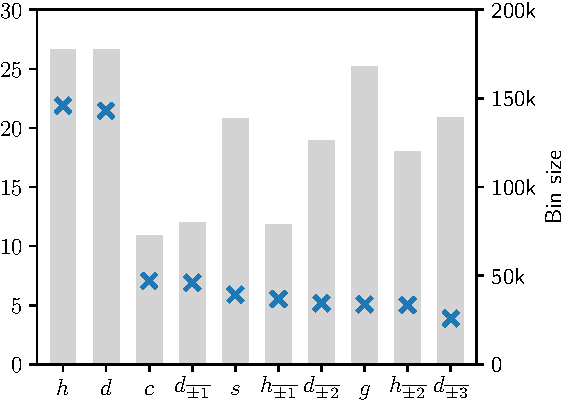
\includegraphics[scale=.75]{figures/OT/graph_features.pdf}
    \caption{Analysis of trained neural dependency parsers from \citet{FalenskaKuhn2019}, aggregating results from nine treebank training experiments (Ancient Greek, Arabic, Chinese, English, Finnish, Hebrew, Korean, Russian and Swedish): impact (blue crosses) of the information from words in various functional positions (occurring with a frequency plotted by the gray bars) on the prediction score of a multi-layer perceptron for a dependency arc in a graph-based dependency parser. The position types compared are the following: heads ($h$), dependents ($d$), children of $d$ ($c$), siblings ($s$), grandparents ($g$), $h,d_{\overline{±i}}$ tokens at distance $±i$ from $h$ or $d$ which are none of $h, d, c, s$, or $g$.}
    \label{fig:impact-plot}
\end{figure}


\figref{fig:impact-plot} shows a diagnostic analysis of the neural model that emerged from training on treebanks for nine languages.
The model was specifically trained to decide whether two given tokens in a sentence should stand in a head-dependent relation, taking into account all tokens in the sentence. For the trained model, it is possible to quantify what impact on the decision the model attributes to individual tokens in the data.\footnote{The paper introduces a special normalized measure for the impact of specific word representations on the prediction.}  For the analysis shown in \figref{fig:impact-plot}, the token impact was systematically aggregated based on the position of the token in the syntactic gold-standard configuration, as labeled in the treebank. (This information is not available to the model itself.)
The blue crosses in the diagram indicate what impact the model itself has decided to assign to tokens in the various configurational positions.  The two tokens with the greatest impact are -- as one would expect -- the head ($h$) and the dependent ($d$) themselves.  But other tokens in the sentence have an impact too.
The gray bars represent the frequency of tokens in the various configurational positions in the training corpora.  In a structurally uninformed model, our expectation would be that the impact of certain types of tokens correlates with their frequency, so the blue crosses should be high on the tall gray bars and low on the short bars. The diagram reveals that the parser has for instance learned from exposure to data to be substantially more sensitive to the children of dependents ($c$) than to siblings ($s$), although the latter occur much more frequently in the training data.\footnote{It should be noted that there is no delimitable locus in the model's parameter space where this information is represented -- but based on the theoretically informed diagnostic tests, we can observe that whatever the model has learned correlates with the distinction.} In fact, the neural model with its self-induced internal representation achieves a better prediction quality than the best classical machine learning models, for which carefully designed configurational features are provided. Since direct information about the representational configuration is not in the input representation that the parser receives in training or application, we have an indication that the emerging internal, connectionist representation does encode implicit knowledge about important aspects of functional structure. 

\largerpage
The linguistic questions that can be addressed with the dependency parsing example are relatively limited, but it is conceivable to generalize the approach to a more complex interplay of factors affecting linguistic expressions.
Diagnostic tools of this kind may thus provide an informed view on the ability of a connectionist model to pick up patterns for which a theory of syntax has posited symbolic abstractions -- capturing their systematic significance.
A central challenge for theoretical interpretability of the models' predictive capacity is to further develop the diagnostic machinery for disentangling the overlaid effects of very different knowledge sources.\footnote{To make progress in this process of disentangling, it is necessary to cross long-established disciplinary boundaries that provided clear-cut subspaces in the study of language, text and corpora of discourses from specific contexts: theory of grammar with its subdisciplines, psycholinguistics, sociolinguistics, but also literary studies, media studies, etc.; many relevant patterns fall into the realm of scholarly disciplines that do not study language and text \emph{per se}, such as cultural studies, history and social science. The delimited subspaces have so far justified convenient idealizations in the working assumptions -- in the theory of grammar for example the idealizing assumption of a shared body of grammatical and lexical knowledge that makes up the linguistic competence of all native speakers of language X. 
An extra challenge comes from the divergent methodologies that have developed in the subfields as a response to the very distinct idealizations; this becomes clear in work in subareas of digital humanities and computational social science which has recently explored corpus-based modeling techniques for addressing research questions from literary studies \citep{Kuhn-Springer} or political science \citep{pado-etal-2019-sides}. Considerable effort is needed to appropriately incorporate findings from computational models in the respective question contexts and theoretical frameworks \citep{CRETA-book}.}


\section{Conclusion: Epistemological considerations}
\label{sec:OT:conclusion}

Optimality Theory was introduced to the study of language in the 1990s as a symbolic description framework for linguistic representations which can make stronger empirically testable predictions about the human language faculty than a classical formal grammar. It can be seen as an attempt to overcome an epistemological limitation of the established formalisms underlying most work in linguistics. The limitation affects plain rewrite systems from the Chomsky hierarchy as much as extensions such as for instance transformational systems, tree-adjoining grammars and unification-based grammars.

\begin{sloppypar}
With a classical framework, the predictions that can be tested ``directly''\footnote{``Directly'' is set in scare quotes, since what goes through as direct empirical evidence in linguistic work always depends on methodological preassumptions that a community agrees on. The nature of language data in communication is such that very few event types are truly observable in a direct way. However, appeal to certain theoretical constructs and certain contextually triggered inferences is typically considered uncontroversial since they are orthogonal to research questions under debate.} against empirical observations are always tied to the formal grammar for a particular language, i.e., a specific instantiation of the class of formal systems, for example, a specific context-free grammar $G_{137} = \langle N_{137}, \Sigma_{137}, P_{137}, S_{137}\rangle$ with a concrete set of non-terminal symbols, terminal symbols, rewrite rule productions and start symbol (and similarly for more expressive grammar formalisms).
\end{sloppypar}

One such instantiation is typically viewed as a scientific model for (aspects of) the grammatical competence of speakers of, say, Japanese, Swahili or English. The formal system predicts a set of terminal strings, which can be experimentally compared against the linguistic behavior of competent speakers. A grammatical theory about a range of phenomena, e.g., in Japanese, is then falsifiable in the sense of \citet{Popper1959}\footnote{Falsifiability is a prerequisite for a theory with any predictive power.} because it is conceivable that relevant types of terminal strings predicted to be excluded from the formal language according to the theory \emph{do} in fact occur in an experiment (potentially using corpus studies that compare against very similar string types predicted to be included).\footnote{Most theories of grammar work with the stronger assumption that (some part of) the internal symbolic structures used by the formalism also represent relevant aspects of meaning, i.e., they can be viewed as logical forms. This provides an additional basis for testable predictions; the experiment then has to access speakers' (and listeners'/readers') interpretation of given strings. What is directly testable are however still the system's predictions for one fully parametrized (language-particular) instance of the grammar formalsm.} The theoretical scope is however rather limited: if $G_{137}$ fails to predict an empirically observable opposition of acceptable vs.\ unacceptable data in Japanese, all that the theorist can conclude is that some aspect in the specification of this formal grammar has been inappropriate.  When there are multiple ways of fixing the problem (e.g., by different strategies of introducing additional non-terminal symbols in a variant $G_{137}'$ and by modifying some existing productions and adding some new ones in $G_{137}''$), there is no theoretically forceful way of distinguishing between them. Assume for the sake of the argument that only one of the modified grammars makes structural similarities with Korean, which is modeled in some grammar $G_{214}$, explicit. As long as the other modified formal grammars predict the same formal language, a theoretically well-founded statement differentiating between the options cannot be made (for lack of falsifiability).

In contrast to classical formal systems, an OT system can make testable predictions for quite a different type of experiment: the theory implemented in a particular OT system, with a spelled-out candidate generation function \emph{Gen} and a set of rankable constraints \emph{Con}, does not predict a single formal language, but -- via the factorial typology implied by all possible rankings of \emph{Con} -- a whole class of formal language approximations of natural languages. Fully formalized OT systems come with a spelled-out empirical learning algorithm (\citealt{TesarSmolensky1998} and subsequent work in the community), which provides the basis for falsifiability of a theory about the human language faculty as such: %(of course, focusing on some selection of linguistic phenomona):
a formal OT system predicts how a learner of any specific language in their learning behavior responds to exposure to language behavior by adult speakers of the language in question.\footnote{Adult behavior is assumed to be observed in contexts that provide enough extra-linguistic clues to support inferences about the intended meaning where there is ambiguity.} A concrete OT system can thus be falsified by evidence from \emph{any} of the languages of the world: a particular observed adult language behavior could in principle trigger a sequence of constraint rerankings that make it impossible for the learner to converge on the constraint ranking needed for this language. If this is the case for some conjectured theory (with a constraint set, etc.) and observed language data, then the theory of some part of the human language faculty counts as falsified.

\begin{sloppypar}
Of course, most research communities employing classical formalisms, including the LFG community, have established agreed-upon meta principles and methodological research practices which effectively ensure that empirical evidence from a particular natural language is accepted by the community as evidence affecting \emph{all} formal systems adhering to the shared conventions (to continue with our context-free grammar illustration, the theory could be characterized as the set of formal grammars $\{ G_i$ $ | $ the components of $G_i$ satisfy all meta principles $\}$). There are countless examples of such meta principles: X-bar theory, extended projections, the concept of lexical redundancy rules, constraints on legitimate transformations in a derivational framework, a universal layering of functional projections, etc. With such principles it becomes possible that the grammatical theory constituted by the meta principles is falsified by language-particular evidence. Even the language learning/acquisition problem has been formulated on the basis of such framework, presumably most prominently in the Principles-and-Parameters theory \citep{chomsky1981lectures}: the learner (guided by some language acquisition device that is assumed to be part of the cognitive equipment) has the task of adjusting a number of free parameters in an otherwise highly constrained innate grammatical system -- in response to observed linguistic behavior by adult speakers. (A rigorous formalization as for OT learning algorithms is typically not provided.)
\end{sloppypar}

However, although sophisticated research practices have been established that ensure a far-reaching consensus about plausible meta principles assumed in a community, the epistemological relationship between a particular instantiation of the meta framework (say, formal grammar $G_{137}$ for Japanese) and the framework itself, with its meta principles, remains contestable. Typically, the representational constructs developed to capture generalizations across natural languages have been established in a long process of cautious plausible reasoning -- yet it is almost always conceivable that there are alternative, empirically indistinguishable ways of predicting surface-level divergences across languages. To explain unexpected patterns in some language X, a modification in the formulation of one or another meta principle could be made, or idiosyncratic lexical knowledge could be posited.
The falsifiability issue of general theoretical statements is not completely resolved by the assumption of meta principles. This circumstance explains in part why there have been many controversial debates about the representational locus for capturing cross-linguistic variation in a phenomenon -- take for instance Binding Principles, which one might construe along a configurational tree structure or along a functional hierarchy \citep{AsudehDalrymple2006}. In the same vein, a re-occurring type of argument against specific linguistic accounts is the accusation for overly strong theory-internal assumptions. In other words, it happens quite frequently that members of a research community develop reservations with respect to the falsifiability of parts of the established consensus framework.\footnote{Given the underdetermination of theories of grammar by direct empirical evidence, aesthetic arguments regarding the simplicity of a theory are often advanced, most notably in Minimalism \citep{chomsky1995the-minimalist}. But even this strategy cannot escape controversies, since there are different possible starting points for seeding a theoretical accounts in fundamental propositions.}

As just noted, OT can be technically seen as the move towards an approach that meets higher standards of falsifiability (when fully formalized). One may ask oneself then why it has not replaced classical formalisms in mainstream linguistic research?  \sectref{sec:OT:after-peak} discussed this question under the perspective of the concrete course of research activities in the 1990s and 2000s. But there are also relevant meta-theoretical considerations: since most aspects of representational choice in linguistic modeling are not directly observable (only the linear sequence of surface units of expression and semantic entailments of the content of utterances are directly observable), the space of possible OT theories remains vastly underdetermined. This means that (unless a community decides to change their research paradigm completely), plausible argumentation for abstract intermediate representations remains an important part of linguistic theorizing.  And since substantial groundwork in linguistic research has always lain in the systematic capturing of regularities in variation patterns for particular languages, the justification for the use of classical formalisms has not disappeared.  By choosing a strict ranking approach over violable constraints captured in terms of established symbolic representations, the OT endeavor was from the outset designed to stay connected with work using the classical formalisms; the effect of relevant constraints on a phenomenon under consideration can be calculated in manually constructed tableaux.\footnote{As was discussed in \sectref{sec:OT:more-recent-developments}, recent machine learning approaches open up alternative avenues for modeling human language behavior. Computational models incorporating a very large parameter space can be trained on large corpora to achieve higher prediction accuracy on most tasks; however, the emerging representations (in the hidden layers of ``deep'' neural network models) provide no direct basis for a falsifiable theory of aspects of linguistic competence. Some connection to hypotheses that can be expressed symbolically seems to be indispensible.}  Insights from a specific OT account may thus feed back into the more general debate of what are appropriate theoretical constructs for systematically capturing a  particular aspect of linguistic knowledge.

Against this background, the most important contribution of OT to generative linguistics might have been to increase the awareness in (part of) the community that a comprehensive, falsifiable account of the human language faculty has to include a formalized account of learnability of language from exposure to data. 

\sloppy
\printbibliography[heading=subbibliography,notkeyword=this]
\end{document}
